\documentclass[12pt,a4paper]{article}

\usepackage[T1]{fontenc}
\usepackage[utf8]{inputenc}
\usepackage[hungarian]{babel}
\usepackage{lmodern}
\usepackage{geometry}
\usepackage{setspace}
\usepackage{hyperref}
\usepackage{enumitem}
\usepackage{longtable}
\usepackage{array}
\usepackage{microtype}
\usepackage{url}
\usepackage{seqsplit}
\usepackage{graphicx}
\usepackage{float}
\usepackage{tikz}
\usetikzlibrary{shapes.geometric, arrows.meta, positioning}
\usepackage{xcolor}
\usepackage{listings}

\lstset{
    basicstyle=\ttfamily\footnotesize,
    keywordstyle=\color{blue}\bfseries,
    stringstyle=\color{orange},
    commentstyle=\color{green!50!black},
    breaklines=true,
    frame=single,
    backgroundcolor=\color{gray!5},
    showstringspaces=false,
    captionpos=b,
    aboveskip=1em,
    belowskip=1em,
    extendedchars=true,
    literate={á}{{\'a}}1 {é}{{\'e}}1 {í}{{\'i}}1 {ó}{{\'o}}1 {ö}{{\"o}}1 {ő}{{\H{o}}}1 {ú}{{\'u}}1 {ü}{{\"u}}1 {ű}{{\H{u}}}1 {Á}{{\'A}}1 {É}{{\'E}}1 {Í}{{\'I}}1 {Ó}{{\'O}}1 {Ö}{{\"O}}1 {Ő}{{\H{O}}}1 {Ú}{{\'U}}1 {Ü}{{\"U}}1 {Ű}{{\H{U}}}1
}

\lstdefinelanguage{json}{
    basicstyle=\ttfamily\footnotesize,
    string=[s]{"}{"},
    stringstyle=\color{orange},
    comment=[l]{:},
    commentstyle=\color{black},
}

\newcolumntype{L}[1]{>{\raggedright\arraybackslash\hspace{0pt}}m{#1}}
\newcommand{\subfile}[1]{\path{#1}}

\geometry{margin=2.5cm}
\onehalfspacing

\begin{document}

\begin{titlepage}
    \begin{center}
        \vspace*{1cm}
        
        \Large
        \textbf{Budapesti Műszaki és Gazdaságtudományi Egyetem} \\
        \textbf{Villamosmérnöki és Informatikai Kar} \\
        \textbf{Irányítástechnikai és Informatika Tanszék}
        
        \vspace{4cm}
        
        \huge
        \textbf{LLM-ALAPÚ ÉRTÉKELŐRENDSZER HALLGATÓI PROGRAMOZÁSI FELADATOKHOZ}
        
        \vspace{1.5cm}
        
        \LARGE
        ÖNÁLLÓ LABORATÓRIUM
        
        \vfill
        
        \begin{minipage}[t]{0.45\textwidth}
            \flushleft
            \textbf{Konzulens:} \\
            Karsa Zoltán István \\
        \end{minipage}
        \hfill
        \begin{minipage}[t]{0.45\textwidth}
            \flushright
            \textbf{Készítette:} \\
            Kilián Marcell András \\
        \end{minipage}
        
        \vspace{2.5cm}
        
        \Large
        Budapest \\
        2026
        
    \end{center}
\end{titlepage}

\tableofcontents
\newpage

\section{Bevezetés és projektcélok}
\label{sec:bevezetes}
Ez a dokumentum egy Python nyelven kidolgozott, LLM-alapú (Large Language Model) kódértékelő rendszer technikai részleteit és működését ismerteti. A megoldás elsődleges célja a hallgatói forráskódok automatizált feldolgozása, azok szakmai szempontok szerinti kiértékelése, valamint szöveges visszajelzés és egy 0--100 közötti pontszám előállítása.

Az LLM-alapú megközelítés alkalmazását az indokolja, hogy a hagyományos statikus elemző eszközök nehezen kezelik a hallgatói kódokban megjelenő egyedi logikai konstrukciókat. Ugyanakkor a tapasztalat azt mutatja, hogy a kisebb paraméterszámú vagy ingyenes modellek gyakran nem megfelelő formátumban, például szintaktikailag érvénytelen JSON-struktúrával, válaszolnak, ami akadályozza az automatizált feldolgozást. A fejlesztett eszköz éppen ezeket a strukturális hiányosságokat hivatott áthidalni robusztus validációs és javító mechanizmusaival.

\subsection{A megvalósítás fókuszpontjai}
\label{sec:fokuszpontok}
A projekt implementációja során számos kihívást kellett áthidalni, amelyek elsősorban a nyelvi modellek működési sajátosságaiból fakadnak. A fejlesztés fókuszában a hallgatói forráskódok automatizált feldolgozása állt, különös tekintettel az olyan kis méretű, egyedi algoritmusokra, amelyek a hagyományos statikus elemzők számára nehezen értelmezhetők.

\section{Hagyományos és AI-alapú kódértékelők összehasonlítása}
\label{sec:hagyomanyos_vs_ai}
Az oktatási célú kódértékelő rendszerek piaca hagyományosan a statikus és dinamikus elemzőeszközökre épülnek, amelyek kiválóan alkalmasak ipari környezetben, azonban az oktatás speciális igényeivel gyakran nehezen birkóznak meg. A hallgatói kódok értékelésének kihívása abban rejlik, hogy a diákok gyakran a várt algoritmustól teljesen eltérő, kreatív vagy éppen hibás, de a jó irányba mutató megoldásokat adnak be. Hagyományos és mesterséges intelligencia alapú kódértékelők összehasonlítása: A hallgatói algoritmusok automatizált kiértékelése évtizedes kihívás a számítástudomány oktatásában \cite{ihantola2010review}. A hagyományos tesztelési keretrendszerek (mint például a Java nyelv esetén használt \textit{JUnit} \cite{junit}) egy adott szoftveregység izolált, determinisztikus tesztelésére lettek kitalálva. Ezen keretrendszereknél a fejlesztő (esetünkben az oktató) előre megírja a bemeneti adatokat és az elvárt kimenetet. A hallgatói kód kiértékelésénél a JUnit egyszerűen lefuttatja a feladatot és ha a kimenet megegyezik a várttal, a teszt sikeres, ellenkező esetben pedig sikertelen. Ennek hatalmas korlátja, hogy teljesen bináris és vak a kód szerkezetére: ha a hallgató megoldása 99\%-ban jó, de az utolsó sorban elfelejtett egy sortörést (\texttt{\textbackslash n}) kiírni, a JUnit azonnal 0 pontot ad. Emellett biztonsági kockázatokat is rejt, hiszen a hallgatói kód (amely akár rosszindulatú memóriaszivárgást vagy végtelen ciklust is tartalmazhat) ténylegesen lefut a szerveren.

\subsection{Hagyományos dinamikus és statikus kódellenőrzők}
A hagyományos kódértékelés leggyakoribb formája a \textbf{dinamikus tesztelés}, amelyet leginkább a \textit{JUnit} vagy hasonló egységtesztelő (unit test) keretrendszerek képviselnek. Ezek a tesztek előre definiált bemenetekkel hívják meg a hallgatói függvényeket és szigorúan ellenőrzik a visszaadott kimenetet. A legnagyobb hátrányuk a hagyományosan alkalmazott zéró tolerancia\footnote{A rendszer a legkisebb, az üzleti logikát nem feltétlenül érintő eltérés (például egy plusz szóköz a konzolos kimenetben) esetén is azonnal hibásnak minősíti az egész megoldást.} elve. Bár a modern tesztkeretrendszerekben a kimenet-normalizálással (például felesleges szóközök és soremelések reguláris kifejezésekkel történő eltávolításával) vagy rugalmas összehasonlító függvények írásával ez a merevség enyhíthető, ha egy hallgató megoldása logikailag ugyan helyes, de egy apró kimeneti elírás (például egy elvárt formázási karakter hiánya) miatt a mintaillesztés mégis elbukik, a naiv dinamikus tesztelők továbbra is teljesen hibásnak értékelhetik a megoldást. Hasonlóan, ha a kód egy kisebb szintaktikai hiba (például egy elfelejtett pontosvessző) miatt le sem fordul, a dinamikus tesztelők egyáltalán nem képesek értékelni a kód mögötti algoritmikus gondolatmenetet.

Ezzel szemben a \textbf{statikus elemzők}, mint például a \textit{SonarQube} vagy a különböző linterek, a kód lefutása nélkül, a forráskód absztrakt szintaxisfáját (AST) és egyéb szemantikus tulajdonságait vizsgálják. Ezek az eszközök rendkívül hatékonyak a kódminőség javításában (például a ciklomatikus komplexitás mérésére, kódolási konvenciók és stílusirányelvek megsértésének felderítésére, valamint potenciális biztonsági sebezhetőségek és kódismétlések azonosítására). Azonban a statikus elemzők egyáltalán nem értik a feladat egyedi specifikációját. Bár képesek ellenőrizni bizonyos strukturális kényszereket (például hogy a kód tartalmaz-e ciklust, rekurziót vagy konkrét osztályokat), önmagukban nem képesek eldönteni, hogy a hallgató algoritmusa szemantikailag helyes-e (például hogy valóban egy bináris keresőfát épít-e fel, vagy csak egy egyszerű tömböt használ a háttérben), pusztán azt jelzik, hogy a megírt kód tiszta-e\footnote{Olyan forráskód, amely könnyen olvasható, karbantartható és szigorúan követi az adott programozási nyelv elfogadott konvencióit.} vagy sem.

\subsection{Az LLM-alapú kódértékelők előnyei az oktatásban}
A nagy nyelvi modellekre (LLM) épülő értékelő rendszerek egy paradigmaváltást hoznak a kódellenőrzésben, mivel egyfajta virtuális tanársegédként\footnote{A szoftver nem csupán bináris (jó vagy rossz) döntést hoz, hanem képes rugalmasan megérteni a diák szándékát és konstruktív, emberi nyelven megfogalmazott magyarázatot adni a hibákra.} működnek. Ezek a modellek nem a szigorú karakteres egyezést vagy a szintaxisfát vizsgálják, hanem képesek megérteni a hallgató \textit{szándékát} a kód alapján.

Az AI-alapú értékelés legnagyobb pedagógiai előnye a részpontszámok (partial credit) osztása. Ha egy hallgató egy kiváló algoritmust tervezett, de elvétett egy indexelést egy tömbben, az LLM képes felismerni a helyes alapkoncepciót és a hibára történő figyelmeztetés mellett megadni az érdemi pontszámot. Ezen felül az LLM-ek szöveges, emberi nyelven megfogalmazott magyarázatot is képesek generálni, amely azonnali, személyre szabott visszajelzést (feedback-et) ad a hallgatónak arról, hogy miért nem optimális a megoldása és hogyan javíthatna rajta. Ez a fajta szemantikai megértés teszi az AI-alapú rendszereket nagyságrendekkel rugalmasabbá a hagyományos megoldásoknál.

\section{Nagy Nyelvi Modellek (LLM) Alapfogalmai}
\label{sec:llm_alapok}
Mielőtt rátérnénk a rendszer architektúrájára és a mérési eredményekre, érdemes röviden tisztázni azokat a fogalmakat és technológiák működését, amelyekre a kódértékelő megoldás épül.

\subsection{Működési elv és a Transformer-architektúra}
A nagy nyelvi modellek (Large Language Models) olyan mesterséges neurális hálózatok, amelyeket hatalmas mennyiségű szöveges adatokon tanítottak be. Modern változataik szinte kivétel nélkül az úgynevezett Transformer-architektúrára épülnek \cite{vaswani2017attention}, amely figyelemmechanizmusok (attention mechanism) segítségével képes megérteni a szavak és kódrészletek közötti kontextusbeli összefüggéseket, még akkor is, ha azok távol helyezkednek el egymástól a szövegben. A kifejezetten forráskódokon (pl. GitHub repozitóriumokon) előtanított modellek megjelenése ráadásul új dimenziókat nyitott a programozási feladatok megértésében \cite{chen2021codex}. A modell alapvető működési elve a következő token (szótöredék) valószínűségi megjóslása a megelőző kontextus alapján.

\subsection{Alapvető fogalmak: Token, Temperature és Top-P (Nucleus Sampling)}
A nyelvi modellek nem karakterekben vagy szavakban, hanem \textbf{tokenekben} dolgozzák fel az információt. Egy token lehet egy teljes szó, egy szórészlet, vagy programozási nyelvek esetében akár egyetlen szintaktikai jel. A \textbf{kontextus ablak} (context window) határozza meg azt a maximális tokenszámot, amelyet a modell egyszerre képes a memóriájában aktívan tartani és értelmezni. Ha egy hallgatói forráskód és az értékelési útmutató együttes hossza túllépi ezt a határt, a modell "elfelejti"\footnote{A nagy nyelvi modellek működéséből fakadóan a bemeneti (kontextus) ablak fix méretű. Amikor a tokenek száma meghaladja ezt a határt, a legrégebbi -- azaz a szöveg legelején lévő -- tokenek kiszorulnak a modell memóriájából (levágásra kerülnek), így az azokhoz kapcsolódó utasítások vagy adatok elvesznek az elemzés során.} a szöveg elejét.

A kimenet generálásának determinisztikusságát és kreativitását két kulcsfontosságú hiperparaméter szabályozza: a \textbf{temperature (hőmérséklet)} és a \textbf{Top-P (Nucleus Sampling)}.
A temperature a generálás során alkalmazott valószínűségi eloszlás "lapításáért" felel. A $0.0$ értékhez közeli temperature szigorúbb, determinisztikus kimenetet eredményez (mindig a legvalószínűbb szót választja), míg a magasabb értékek (például $0.8$) növelik a kreativitást és egyben a hallucinációk esélyét is.

A \textbf{Top-P} egy eltérő mechanizmus, amely levágja a lehetséges következő szavak listáját (szótárát) egy kumulatív valószínűségi küszöb alapján. Ha a \texttt{Top-P = 0.1}, a modell csak azokat a legesélyesebb tokeneket veszi figyelembe a sorsolásnál, amelyek együttes valószínűsége eléri a 10\%-ot. A maradék, alacsony valószínűségű, "furcsa" szavakat (a statisztikai hosszú farkat) a rendszer egyszerűen eldobja.

Kódértékelési feladatoknál, ahol szigorú szintaktikai (JSON) kimenetet és logikai konzisztenciát várunk, elengedhetetlen a véletlenszerűség minimalizálása. A két paraméter együttes hatását vizsgáló kísérletek rávilágítanak, hogy ha a temperature-t valamilyen okból emelnünk kell (például hogy a modell hosszabb, emberszerűbb magyarázatot írjon), az alacsonyan tartott Top-P (pl. $0.1$) képes kiszűrni a hallucinációkat, így megőrizve az értékelés konzisztenciáját.

\begin{table}[H]
    \centering
    \begin{tabular}{|c|c|c|p{7.5cm}|}
        \hline
        \textbf{Temperature} & \textbf{Top-P} & \textbf{Korreláció (r)} & \textbf{Jellemző viselkedés} \\
        \hline
        0.1 & 0.1 & \textbf{0.640} & Rendkívül stabil, determinisztikus (Optimális) \\
        \hline
        0.1 & 0.9 & 0.620 & Stabil kimenet, minimális szóhasználati varianciával \\
        \hline
        0.5 & 0.1 & 0.632 & Jó kompromisszum: emberibb magyarázatok, stabil JSON \\
        \hline
        0.5 & 0.9 & 0.611 & Inkonzisztens struktúra és logikai tévedések megjelenése \\
        \hline
        0.9 & 0.9 & 0.545 & Súlyos hallucinációk, a kód futásának hibás értelmezése \\
        \hline
    \end{tabular}
    \vspace{0.2cm}
    \caption{\textit{A Temperature és a Top-P paraméterek együttes hatása a tanári értékeléssel való korrelációra. (50 fős hallgatói mintán tesztelve, Mentális Végrehajtás móddal). Jól látható, hogy a magas temperature (0.5) okozta pontosságromlást egy alacsony Top-P érték (0.1) képes tompítani (0.611 helyett 0.632).}}
    \label{tab:temp_topp}
\end{table}

\subsection{Modellek paraméterszáma és a teljesítmény összefüggése}
\label{sec:parameterek}
Az LLM-ek okosságát\footnote{A modell komplex problémamegoldó képessége, kontextusmegértése és a kódokon belüli logikai összefüggések felismerésének pontossága.} és komplexitását nagyban meghatározza a betanított súlyok, azaz a \textbf{paraméterek száma}. Ez a szám azt jelzi, hogy a neurális hálózat hány állítható kapcsolattal rendelkezik. A paraméterszám közvetlen hatással van a modell logikai következtető képességére és arra, hogy mennyire képes megérteni a komplex összefüggéseket egy diák kódjában.

A jelenlegi mérésekben részt vevő modellek paraméterszámai jelentős eltéréseket mutatnak. A nyílt forráskódú \textbf{Llama 3.1 70B} modell 70 milliárd paraméterrel rendelkezik, míg az iparági szintű \textbf{Mistral Large 2} becslések szerint körülbelül 123 milliárd tanulható súllyal operál. Az optimalizált, kisebb méretű, költséghatékony (úgynevezett budget)\footnote{A költséghatékony modellek olyan kisebb architektúrák, amelyeket úgy optimalizáltak, hogy töredék áron és sokkal gyorsabban fussanak, mint az elit kategóriás csúcsmodellek, miközben az egyszerűbb feladatokban megközelítik azok pontosságát.} modellek, mint a \textbf{Claude 3 Haiku} és a \textbf{GPT-4o-mini}, szakmai becslések alapján a 8 és 20 milliárd paraméter közötti tartományban mozognak. Ezzel szemben a csúcskategóriás elit modell, a \textbf{GPT-4o}, a feltételezések szerint rendkívül masszív Mixture of Experts (MoE) architektúrára épül, amelynek paraméterszáma megközelítheti az 1,8 billiót.

A teljesítmény és a neurális hálózat mérete közötti összefüggés (regresszió) a hagyományos kiértékelésnél (Original mód) egyértelműen kimutatható a korrelációs eredményekben. Egy jelentősen nagyobb hálózat, mint például a GPT-4o, sokkal magasabb korrelációt (r=0.75) mutat a tanári pontozással, mivel hatalmas belső tudásbázisának köszönhetően puszta kódelemzéssel is képes átlátni a hallgatói algoritmusok rejtett logikai hibáit. Ezzel szemben, ha a hálózat lényegesen kisebb, az értő olvasási képesség csökken: például a 10 milliárd paraméter körüli Claude Haiku ránézésre\footnote{A modellnek egyetlen lépésben, előzetes logikai lépésekre bontás vagy tesztesetek generálása nélkül kell azonnal kiértékelnie a kódot.} történő pontozásnál szinte teljesen elveszíti a logikai fonalat (r=0.14). 

Fontos mérnöki áttörés azonban, hogy a modell méretéből adódó hátrány drasztikusan csökkenthető a megfelelő, lépésről-lépésre történő instrukciók (Mental Execution mód) alkalmazásával. Ennek során a modellnek teszteseteken kell gondolatban végigvezetnie az adatokat. Ahogy a későbbi mérések igazolják, ezzel a módszerrel egy kisebb hálózat is képes megközelíteni (vagy speciális esetekben felülmúlni) az elit modellek pontosságát, minimalizálva a méretbeli különbségeket.

\section{Tervezés és Architektúra}
\label{sec:tervezes}
A rendszer moduláris felépítésű, ahol az üzleti logika és az értékelési mechanizmusok szétválasztása biztosítja a bővíthetőséget. A főbb komponenseket és a prompt-tervezési elveket az alábbiakban részletezem.

\begin{figure}[H]
    \centering
    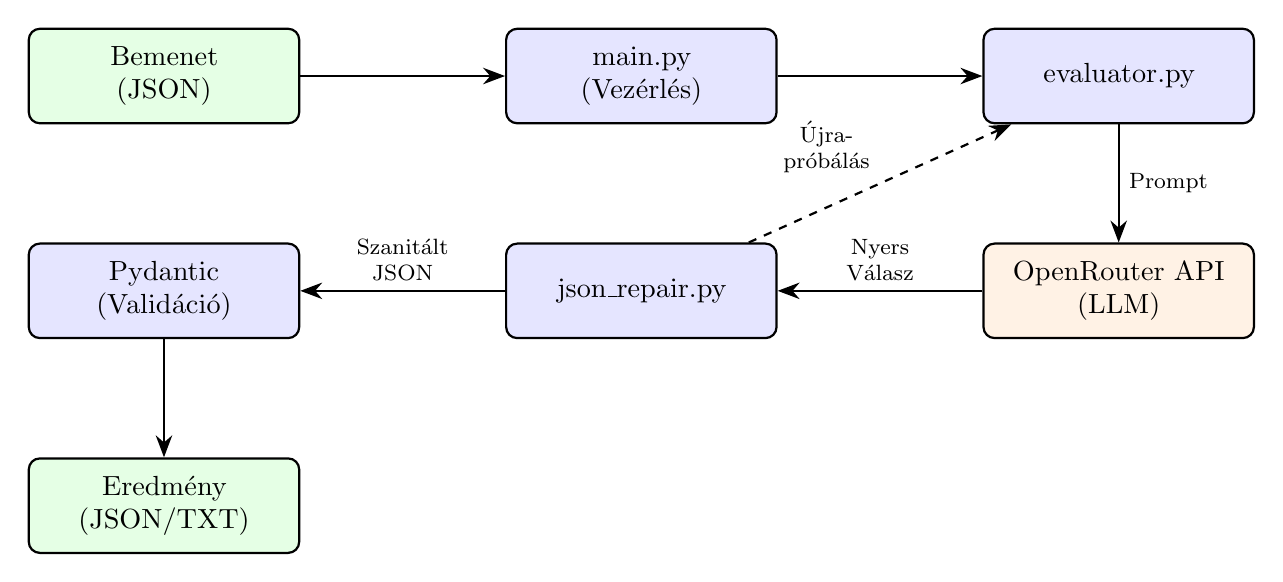
\begin{tikzpicture}[
        node distance=1.5cm and 2.6cm,
        box/.style={rectangle, draw=black, thick, fill=blue!10, text width=3.2cm, text centered, rounded corners, minimum height=1.2cm},
        arrow/.style={-{Stealth[scale=1.2]}, thick},
        labelnode/.style={font=\footnotesize, align=center}
    ]
        % Nodes
        \node (input) [box, fill=green!10] {Bemenet\\(JSON)};
        \node (main) [box, right=of input] {main.py\\(Vezérlés)};
        \node (eval) [box, right=of main] {evaluator.py};
        \node (llm) [box, fill=orange!10, below=of eval] {OpenRouter API\\(LLM)};
        \node (repair) [box, left=of llm] {json\_repair.py};
        \node (pydantic) [box, left=of repair] {Pydantic\\(Validáció)};
        \node (output) [box, fill=green!10, below=of pydantic] {Eredmény\\(JSON/TXT)};

        % Arrows
        \draw [arrow] (input) -- (main);
        \draw [arrow] (main) -- (eval);
        \draw [arrow] (eval) -- (llm) node[midway, right, labelnode] {Prompt};
        \draw [arrow] (llm) -- (repair) node[midway, above, labelnode] {Nyers\\Válasz};
        \draw [arrow] (repair) -- (pydantic) node[midway, above, labelnode] {Szanitált\\JSON};
        \draw [arrow] (pydantic) -- (output);
        \draw [arrow, dashed] (repair) -- (eval) node[midway, above left, labelnode] {Újra-\\próbálás};
    \end{tikzpicture}
    \caption{\textit{A kódértékelő rendszer magas szintű architektúrája és az adatfeldolgozási folyamat.}}
    \label{fig:arch_flowchart}
\end{figure}

\subsection{Fő komponensek}
\label{sec:komponensek}
A szoftverarchitektúra több, jól elkülöníthető felelősségi körrel rendelkező komponensből áll. A belépési pontot a \texttt{main.py} modul jelenti, amelynek feladata a bemeneti adatok kiválasztása, a hallgatói megoldások elemzésének indítása, a teljes kiértékelési ciklus vezérlése, valamint az eredmények végső archiválása. Ennek működését a \texttt{settings.py} konfigurációs fájl támogatja, amely összefogja a rendszer globális paramétereit, beleértve az API-kulcs kezelését, a modellválasztást, az LLM hőszabályozási (temperature) értékeit és a hálózati várakozási időket.

Az értékelő logika magját a \texttt{core} könyvtár moduljai alkotják. Itt kapott helyet az \texttt{evaluator.py}, amely felelős a promptok\footnote{Az a bemeneti szöveg vagy utasításhalmaz, amelyet a felhasználó vagy a rendszer a nyelvi modellnek ad, hogy ez alapján generáljon választ.} dinamikus összeállításáért, az LLM-mel való hálózati interakcióért, valamint a válaszok feldolgozásáért. A kapott válaszok szerkezeti integritását a \texttt{response\_format.py} és a \texttt{response\_models.py} fájlok biztosítják, előbbi a JSON Schema alapú kikényszerítésért, utóbbi pedig a Pydantic keretrendszeren alapuló, típusbiztos validációért felel. Amennyiben a nyelvi modell hibás formátumban válaszol, a \texttt{json\_repair.py} modul kísérli meg a strukturális ellenőrzést és az automatizált javítást. A sikeres kiértékelést követően a \texttt{score\_output\_builder.py} állítja össze a végleges, aggregált pontozási jelentést.

A nyelvi modellek irányításához szükséges sablonok a \texttt{prompts} mappában találhatók. A központi szakmai irányelveket az \texttt{evaluate.txt} határozza meg, míg a hibakezelést a \texttt{repair\_json.txt} és a minőségorientált újrapróbálkozási ciklust vezérlő \seqsplit{retry\_quality\_mode.txt} állományok végzik. Végül a rendszer megbízhatóságának ellenőrzését a \texttt{validation} könyvtár eszközei, \texttt{test\_validation.py} és a \texttt{validation\_analyzer.py} támogatják, amelyek a referenciaadatokkal való statisztikai összehasonlítást teszik lehetővé.

\section{Megvalósítás és Adatstruktúrák}
\label{sec:megvalositas}
A szoftver implementációja során a strukturált válaszok kikényszerítése és a hibatűrő adatkezelés volt az elsődleges szempont. Ez a fejezet a kimeneti sémák evolúcióját és a technikai validációs rétegeket mutatja be.

\subsection{Adatstruktúra és mezőkiépítés}
\label{sec:adatstruktura}
A rendszer JSON-séma (JSON Schema) alkalmazásával garantálja a válaszok strukturális integritását. A válaszséma három fő komponenst tartalmaz. Az első a \texttt{score}\footnote{Azt reprezentálja, hogy a hallgató hány szakmai kritériumot teljesített sikeresen a feladatleírásból.}, amely egy 0--5 közötti belső pontszámot takar, ahol az 5-ös érték a feladat összes kritériumának maradéktalan teljesülését jelzi. Ezt egészíti ki a \texttt{percentage}\footnote{0--100 közötti skálára vetített, hagyományos százalékos megfelelője, amely megkönnyíti az egyetemi oktatási rendszerekkel (például a JPortával) való végső integrációt.} mező, amely a megoldás minőségét tükrözi egy 0--100 százalékos tartományban. A harmadik elem az \texttt{evaluation}\footnote{Strukturálatlan, szabad folyású szöveges mező, ahol a modell elmagyarázza a döntését, rávilágít a hallgatói kód logikai hibáira és javaslatokat tesz a javításra.}, amely egy maximum 600 karakteres, magyar nyelvű szöveges szakmai értékelést biztosít a hallgató számára.

A mezők sorrendjének gyakorlati jelentősége kiemelkedő. A prompt úgy lett kialakítva, hogy a JSON objektumban először a részletes szöveges értékelés (evaluation) kapjon helyet és csak ezt kövesse a numerikus pontszám. Ennek az elrendezésnek az elméleti hátterét a \textit{Chain-of-Thought (CoT)} promptozási stratégia adja \cite{wei2022chain, kojima2022zero}. A megfigyelések és a szakirodalom alapján, ha a nyelvi modell előbb kénytelen megfogalmazni és leírni az érvelését, akkor a később generált aggregált ítélet sokkal konzisztensebb lesz a leírtakkal \cite{nye2021show, wei2022chain, kojima2022zero}. Ha a pontszámot kellene először megadnia, a modell hajlamos lenne véletlenszerűbb ítéletet hozni és a szöveges értékelést ahhoz a helytelen számhoz igazítani.

A rendszer a \texttt{strict} mód mellett alkalmazott karakterlimittel arra kényszeríti a modellt, hogy tömörebb, lényegre törőbb visszajelzéseket adjon. Ez a megközelítés csökkenti a kimeneti entrópiát, mivel a modellnek nem kell döntéseket hoznia a terjedelemről vagy a hangsúlyokról, hatékonyabban képes a szakmai tartalomra fókuszálni.

\subsection{Kimeneti formátum és kiértékelési módok evolúciója}
\label{sec:formatum_evolucio}
A rendszer fejlődése során három alapvetően eltérő megközelítést alkalmaztam a kiértékelésre, amelyek a promptok felépítésében és az elvárt elemzési logikában különböznek.

A \textbf{Sima / Holisztikus (Original) kiértékelési mód} egy magas szintű szemléletet követ, amelyben az LLM a feladatleírás és a forráskód alapján egyetlen lépésben hoz szakmai ítéletet. A válasz csupán a három említett fő adatmezőt tartalmazza. Ez a megközelítés a hallgatói algoritmus szándékolt működésére és a logikai gondolatmenet felismerésére fókuszál. A modell itt rugalmasan kezeli a jelentéktelen szintaktikai hibákat, amennyiben a kód mögötti koncepció alapvetően helyes. Legnagyobb előnye az alacsony latencia, a nagyfokú adaptivitás és a stabil, könnyen feldolgozható JSON-válasz.

A \textbf{Komplex Teszteset-alapú (Testcases) mód} egy sokkal szigorúbb, verifikációs láncot követett. Ennél a módszernél az volt az elvárás, hogy a modell először generáljon teszteseteket, a feladat komplexitásától függően átlagosan 10-15 darabot, majd ezeken a teszteken virtuálisan, lépésről-lépésre futtassa le a hallgatói forráskódot. Az értékelés alapját így nem az algoritmikus szándék, hanem a mérhető teszteredmények szigorú összegzése adta. Bár ez a megközelítés elméletben precízebb, a gyakorlatban a magas fokú szabálykövetés miatt gyakran túl merevnek, gépiesnek\footnote{A modell szigorúan, a kontextus és a hallgatói szándék rugalmas megértése nélkül próbálja kipipálni az előre definiált feltételeket, még akkor is, ha a generált tesztesetek éppen egymásnak ellentmondanak.} bizonyult. A komplex struktúra miatt gyakran idézett elő JSON szintaktikai hibákat és a modell hajlamos volt egymásnak ellentmondó ellenőrzési kritériumokat generálni. Ehhez a bonyolult sémához képest az egyszerűbb, holisztikus formátum sokkal megbízhatóbbnak bizonyult strukturálisan.

A \textbf{Mentális Szimulációs (Mental Execution) mód} az előző kettő ötvözete, fókuszban a Chain-of-Thought (gondolatmenet) megközelítéssel. Ebben a módban a modellnek nem kell kimerítő mennyiségű tesztesetet generálnia, csupán néhány kritikus peremesetet. A feladata, hogy egy emberi tesztelőhöz hasonlóan, sorról-sorra absztrakt módon szimulálja (mintegy fejben végigkövesse) a változók állapotát és ezt a nyomkövetést  le is írja a visszajelzésben. Ez a módszer, melyet a szakirodalom a modellek \textit{scratchpad} (vázlattömb) alapú számítási képességeként is azonosít \cite{nye2021show}, rákényszeríti a kisebb modelleket is, hogy felismerjék a rejtett logikai hibákat ahelyett, hogy felületesen olvasnák el a kódot.

\begin{figure}[H]
    \centering
    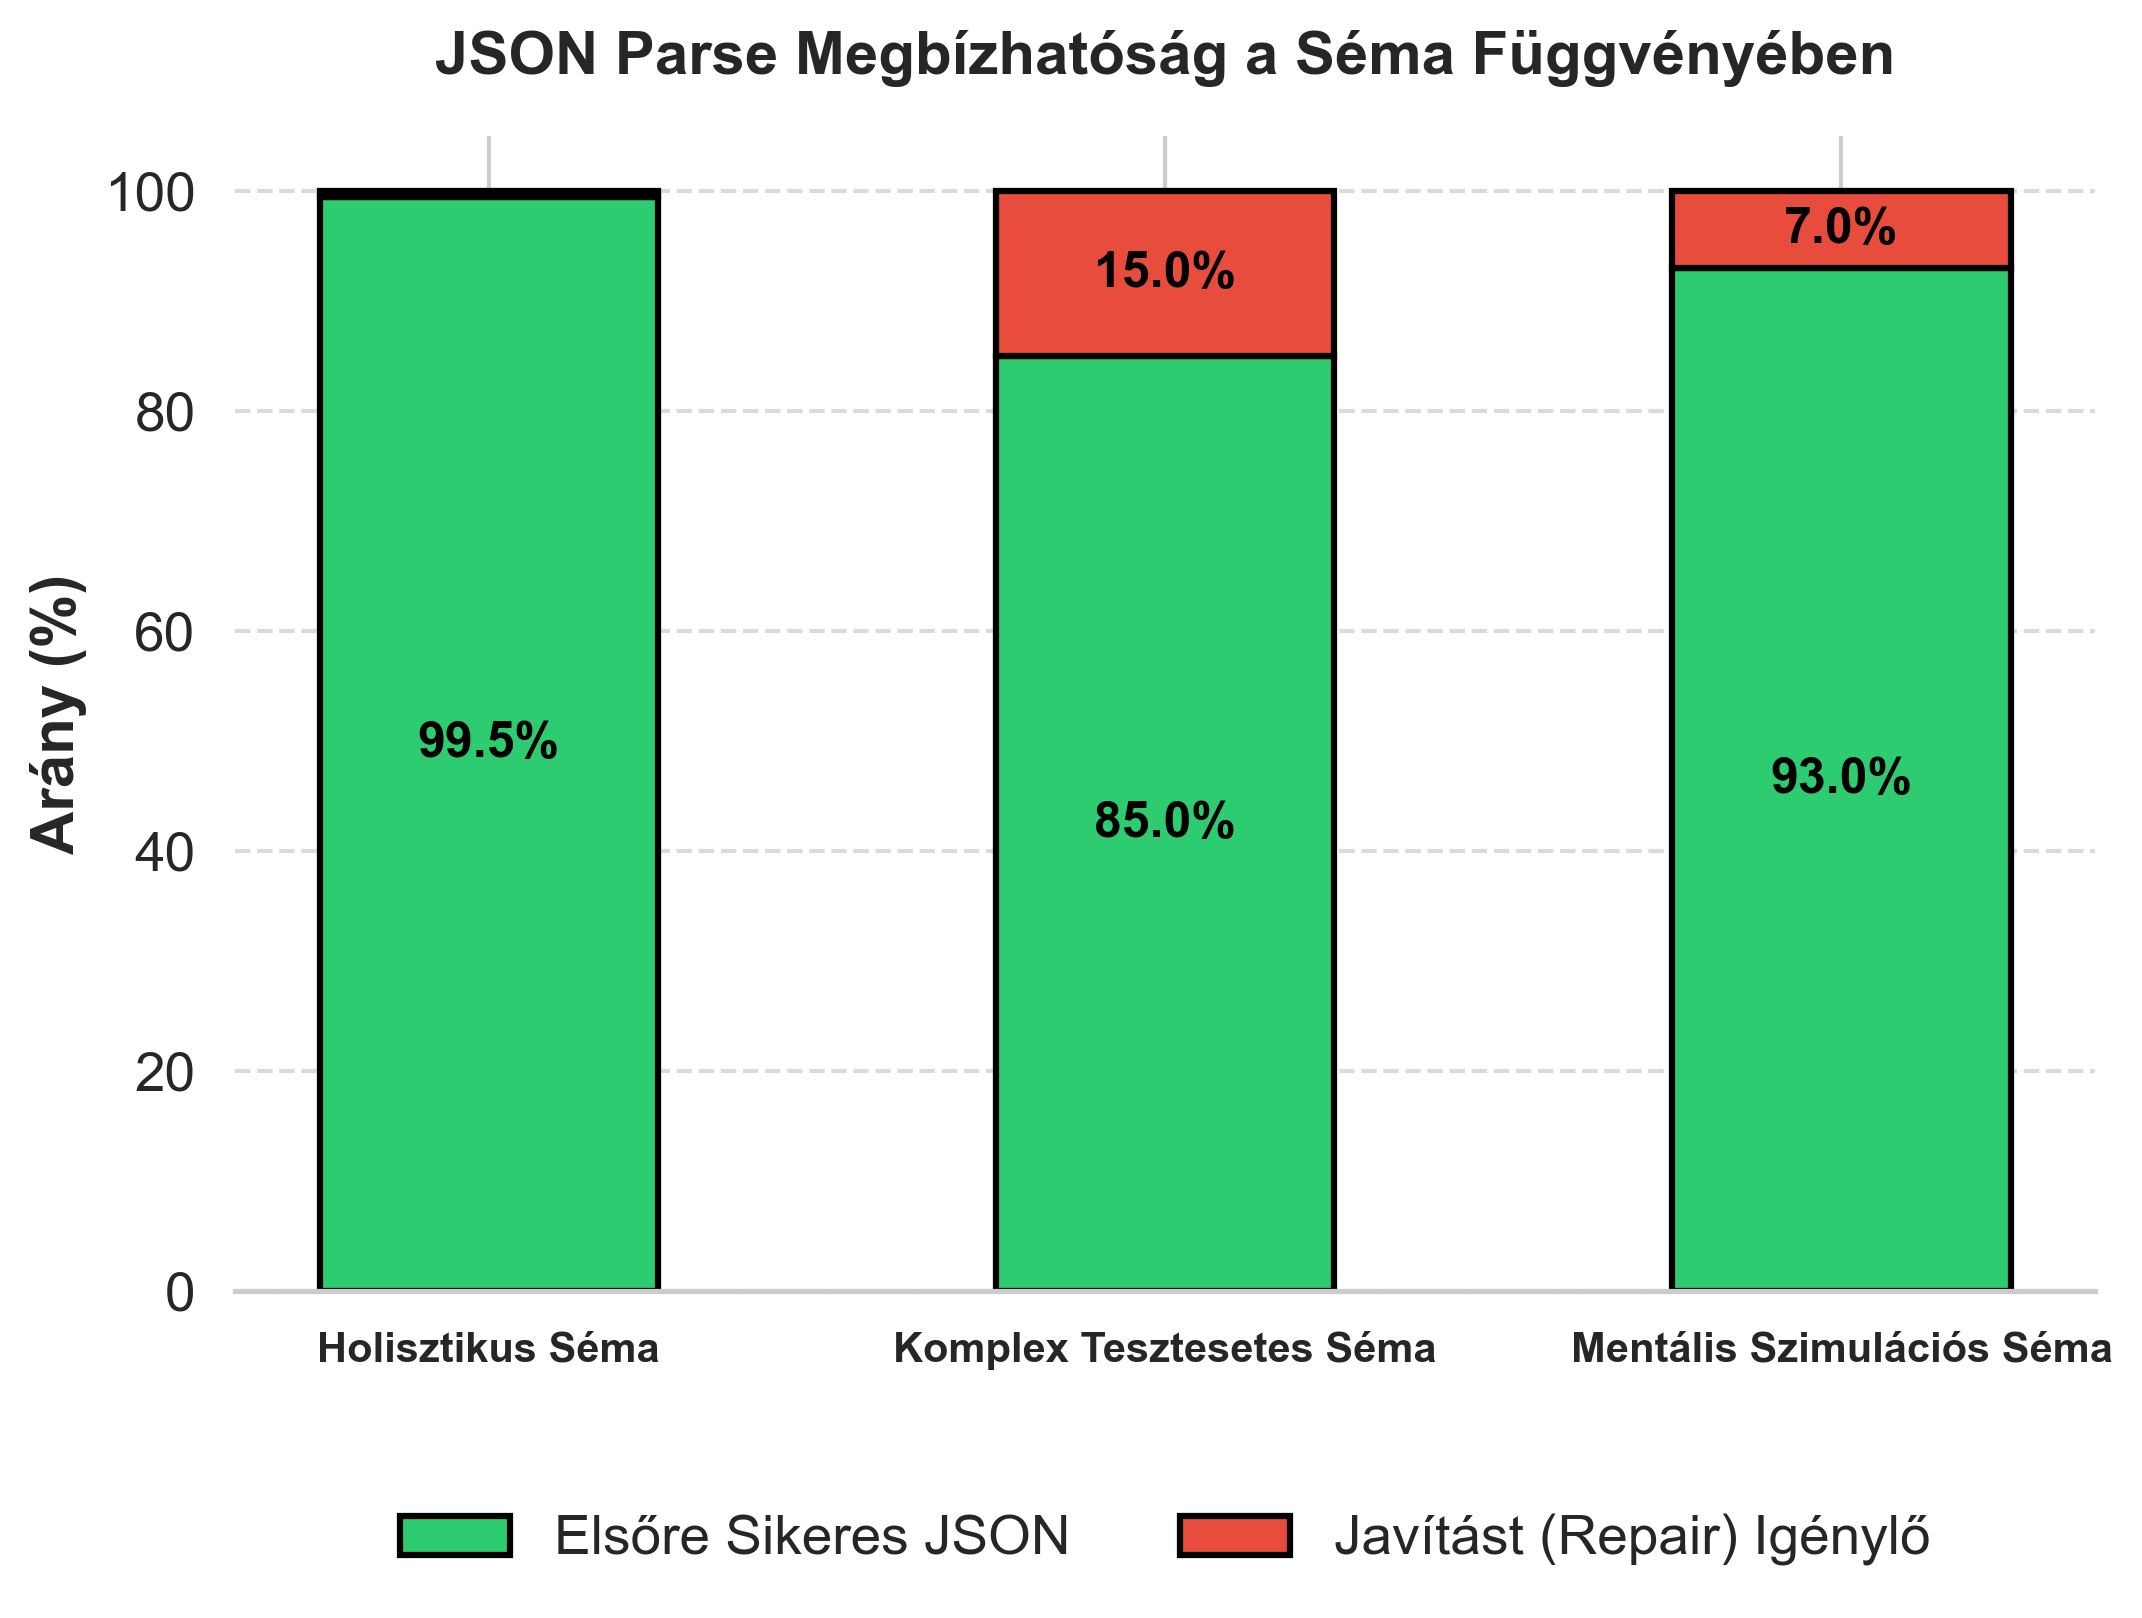
\includegraphics[width=0.8\textwidth]{images/json_reliability.png}
    \caption{\textit{Az LLM-válaszok szerkezeti megbízhatósága. Jól látható, hogy az egyszerűsített holisztikus séma használatával szinte teljesen eliminálhatóak a parser-hibák.}}
    \label{fig:json_rel}
\end{figure}

\subsubsection*{Áttérés a 0--5 pontos skálára}
A fejlesztés egy korábbi szakaszában használt 0--6 pontos skálát a végleges rendszerben egy standard \textbf{0--5 pontos skála} váltotta fel. Ennek oka, hogy az 5-ös skála minden pontja pontosan 20\%-ot ér, ami intuitívabb az LLM és a felhasználók számára is. A korábbi szakaszban az LLM akkor adott 6 pontos értékelést, ha a megoldás minden szempontból hibátlanul és optimálisan teljesítette az elvárásokat. A prompt 5 szakmai kritériumot generál, így a pontszám közvetlenül a teljesített kritériumok számát tükrözi. Ezzel megszűntek a bónusz pont keresése miatti indokolatlanul magas pontszámok.

\subsection{Strukturált kimenet kényszerítése és validáció}
\label{sec:kenyszerites}
A robusztus működés érdekében a bemutatott sémákat több rétegű validáció és javítási mechanizmus védi.

\subsubsection*{JSON Schema és response format}
A \texttt{core/response\_format.py} modul explicit JSON Schema definíciót tartalmaz, amely meghatározza az elvárt mezőket és azok szigorú típusait (például szöveg vagy integer). A séma bekapcsolt strict móddal\footnote{A Strict mód (szigorú mód) az OpenRouter/OpenAI API egy beállítása, amely kényszeríti, hogy a nyelvi modell által visszaadott JSON objektum pontosan, hiánytalanul kövesse a megadott sémát.} kerül az OpenRouter API-hoz, így a modell matematikai kényszer alatt áll, hogy a definiált adatszerkezetet adja vissza.

\subsubsection*{Tisztítás és hibajavítás}
A \texttt{core/json\_repair.py} modul több lépcsős védelmi vonalat biztosít az érvénytelen válaszok ellen. Első lépésként megkísérli a nyers válasz Markdown-blokkokból\footnote{Olyan jelölések, amelyeket a modellek gyakran a kódjuk köré tesznek formázás céljából, de amik egy szigorú JSON feldolgozó (parser) számára szintaktikai hibát okoznak.} való kinyerését, majd a Unicode karakterek\footnote{Univerzális kódolású betűk vagy szimbólumok, amelyek esetenként rosszul (például \u00E1 formátumban) vagy hibás eszképe-eléssel jelennek meg az LLM kimenetében.} tisztítását. Amennyiben az automatikus tisztítás sikertelen, a rendszer felkéri a modellt az eredeti hibaüzenet alapján a javításra. A javító folyamat kizárólag a formátum helyreállítására szorítkozik, az értékelés szakmai tartalmát nem módosítja. A rendszer ezt reguláris kifejezéseken (regex) alapuló szabályokkal valósítja meg, amelyek kizárólag a JSON szerkezet javítására irányulnak, helyreállítják a hiányzó idézőjeleket a kulcsok körül, pótolják a hiányzó zárójeleket, valamint eltávolítják a felesleges vesszőket, miközben a sztringértékek,  a modell által generált szakmai szöveges tartalom, változatlanul maradnak.

\subsection{Alkalmazott Nagy Nyelvi Modellek (LLM) Specifikációi}
A kiértékelő rendszer tesztelése és a benchmark mérések során az OpenAI legmodernebb modelljeit, a \textbf{GPT-4o}-t és a \textbf{GPT-4o-mini}-t (valamint korábban az Anthropic Claude 3 Haiku modelljét) alkalmaztam. 

\subsubsection*{Kontextus ablak (Context Window)}
A kontextus ablak határozza meg, hogy a modell egyszerre mennyi bemeneti adatot képes feldolgozni és a kontextusában aktívan tartani. Mind a GPT-4o, mind a GPT-4o-mini modell \textbf{128 000 tokenes} (körülbelül 300 oldalnyi szövegnek megfelelő) hatalmas kontextus ablakkal rendelkezik. Ez a kiértékelés szempontjából kritikus fontosságú, mivel biztosítja, hogy a teljes feladatleírás, a hallgatói kód és az összetett kiértékelési prompt kényelmesen elférjen a memóriában, akár a tesztesetek dinamikus generálása során is. A Claude 3 Haiku modell esetén ez a méret még nagyobb, 200 000 token.

\subsubsection*{Tanítható súlyok (Paraméterszám) és Tanító adathalmaz}
A modellek belső architektúrájára és méretére vonatkozó pontos adatokat (a tanítható súlyok, azaz paraméterek összegét) az OpenAI zárt forráskódú modellként üzleti titokként kezeli, így hivatalos számok nem állnak rendelkezésre. Ipari becslések alapján a GPT-4o egy hatalmas, valószínűleg billió (Trillion) feletti paraméterszámmal rendelkező MoE (Mixture of Experts) architektúra, míg a GPT-4o-mini egy jelentősen kisebb (milliárdos nagyságrendű), hatékonyságra optimalizált költséghatékony hálózat. 

A modellek betanítása hatalmas, nyilvánosan elérhető webalapú adathalmazokon (szövegek, kódok, matematikai levezetések) történt, amelyet az OpenAI jogvédett és saját fejlesztésű, specifikus adatokkal egészített ki. A modellek (2023. októberi tudásbázis-korláttal) Reinforcement Learning from Human Feedback (RLHF) módszerrel lettek finomhangolva, ami garantálja, hogy a kódértékelés során emberhez hasonló, koherens szakmai indoklásokat generáljanak.

\section{Mérési eredmények és statisztikai elemzés}
\label{sec:meresek}
A rendszer hatékonyságát és pontosságát egy kiterjedt méréssorozat keretében vizsgáltam, amelynek során a hallgatói forráskódokat különböző modellekkel és kiértékelési módokkal (Original, Testcases és Mental Execution) elemeztem. A pontosság mérésére az LLM által adott pontszámok és a manuális tanári értékelések közötti Pearson-féle korrelációs együtthatót ($r$) alkalmaztam. Az LLM-ek nemdeterminisztikus jellegéből adódó varianciák csökkentése érdekében a kiértékeléseket módonként eltérő ismétlésszámmal végeztem el. A Holisztikus (Original) és a Mentális Szimulációs (Mental Execution) módok esetében, amelyek közvetlen szöveggenerálásra épülnek, a kiértékelést minden hallgató kódjára tizenötszörös futtatással (15x) hajtottam végre, és az eredmények átlagát vetettem össze a tanári referenciaértékekkel. A Teszteset-alapú (Testcase) módnál, mivel a tesztgenerálás egyszeri feladat, a tesztfájlok létrehozását tizenötször (15x) próbáltam meg, a sikeres és stabil tesztfájl elmentése után pedig a hallgatói kódok futtatása ezen a fix tesztszkripten egyszeres futtatással (1x) történt meg, hiszen a dinamikus kódvégrehajtás és a pontszám-számítás a homokozóban teljesen determinisztikus.

\subsection{Különböző kiértékelési módszerek teljesítménye}
Az elemzésből világosan kirajzolódik a modell paraméterszáma és az alkalmazott kiértékelési stratégia közötti kapcsolat. Amint a \ref{fig:method_comp}. ábrán látható, az elit modellek (például a GPT-4o) a sima (original) módban képesek a legmagasabb korrelációt elérni, mivel belső kapacitásuk elegendő a logikai hibák azonnali felismeréséhez. Ezzel szemben a kisebb, "budget" kategóriás modellek számára a holisztikus értékelés komoly nehézséget okoz.

Különösen érdekes azonban a mentális szimulációs mód hatása, a Claude 3 Haiku modell esetében ez a lépésről-lépésre történő szimulációs eljárás hatalmas ugrást eredményezett a pontosságban (r=0.707). Míg az Original módban a modell szinte értékelhetetlen teljesítményt nyújtott (r=0.141), a mentális futtatás rákényszerítette a logikai hibák deduktív feltárására, amivel sikeresen hidalta át a paraméterszámból adódó hátrányt.

\begin{figure}[H]
    \centering
    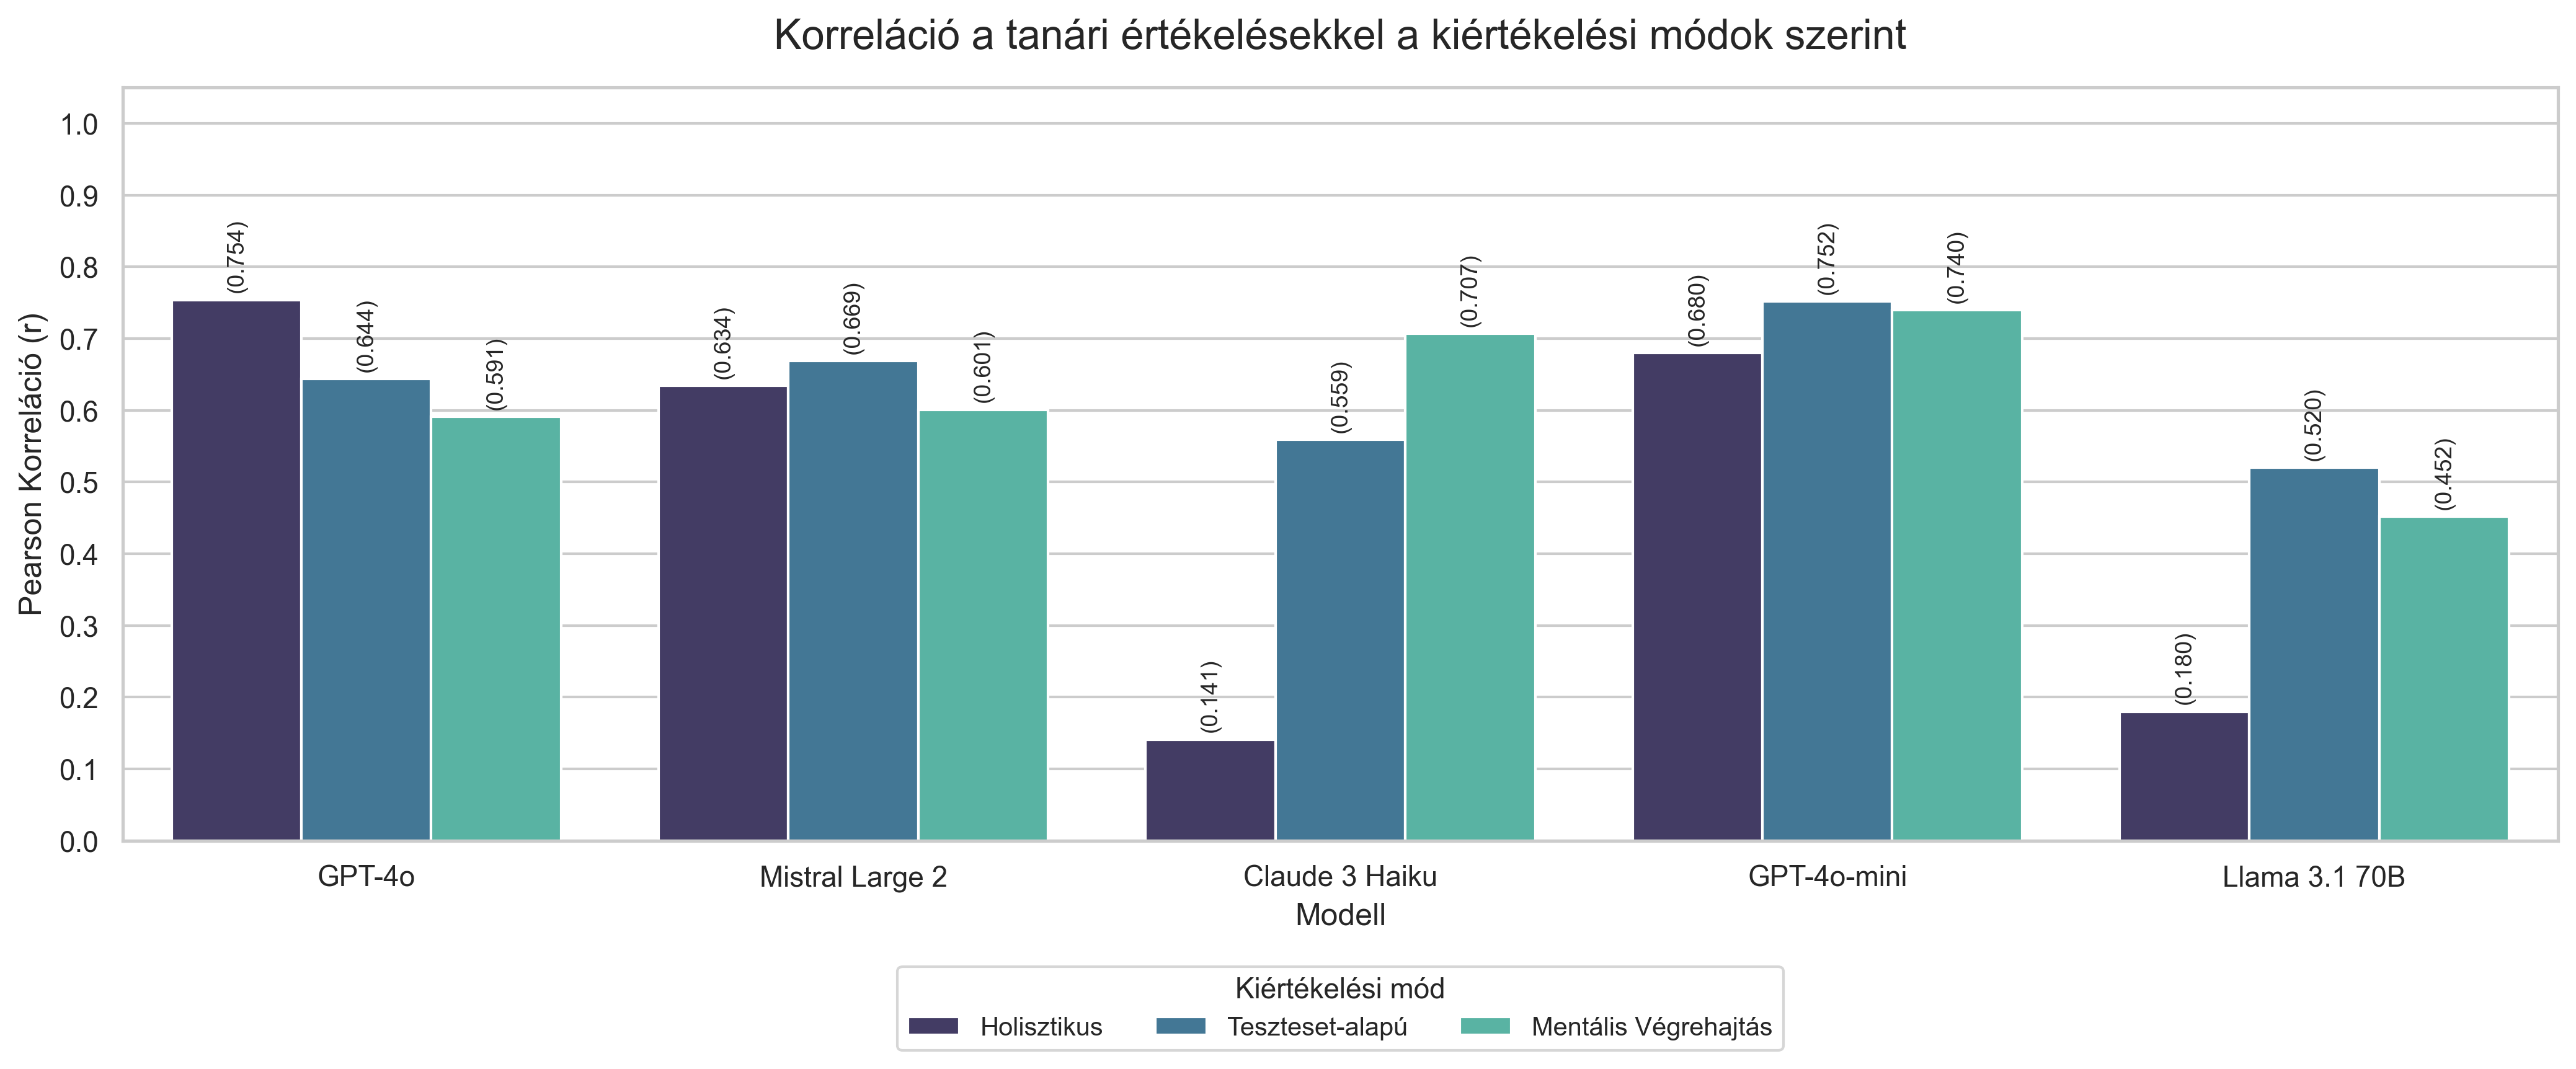
\includegraphics[width=\textwidth]{images/method_comparison.png}
    \caption{\textit{A Pearson-korreláció ($r$) alakulása a tanári pontszámokkal összevetve, a különböző nyelvi modellek és kiértékelési módok esetében.}}
    \label{fig:method_comp}
\end{figure}

\begin{figure}[H]
    \centering
    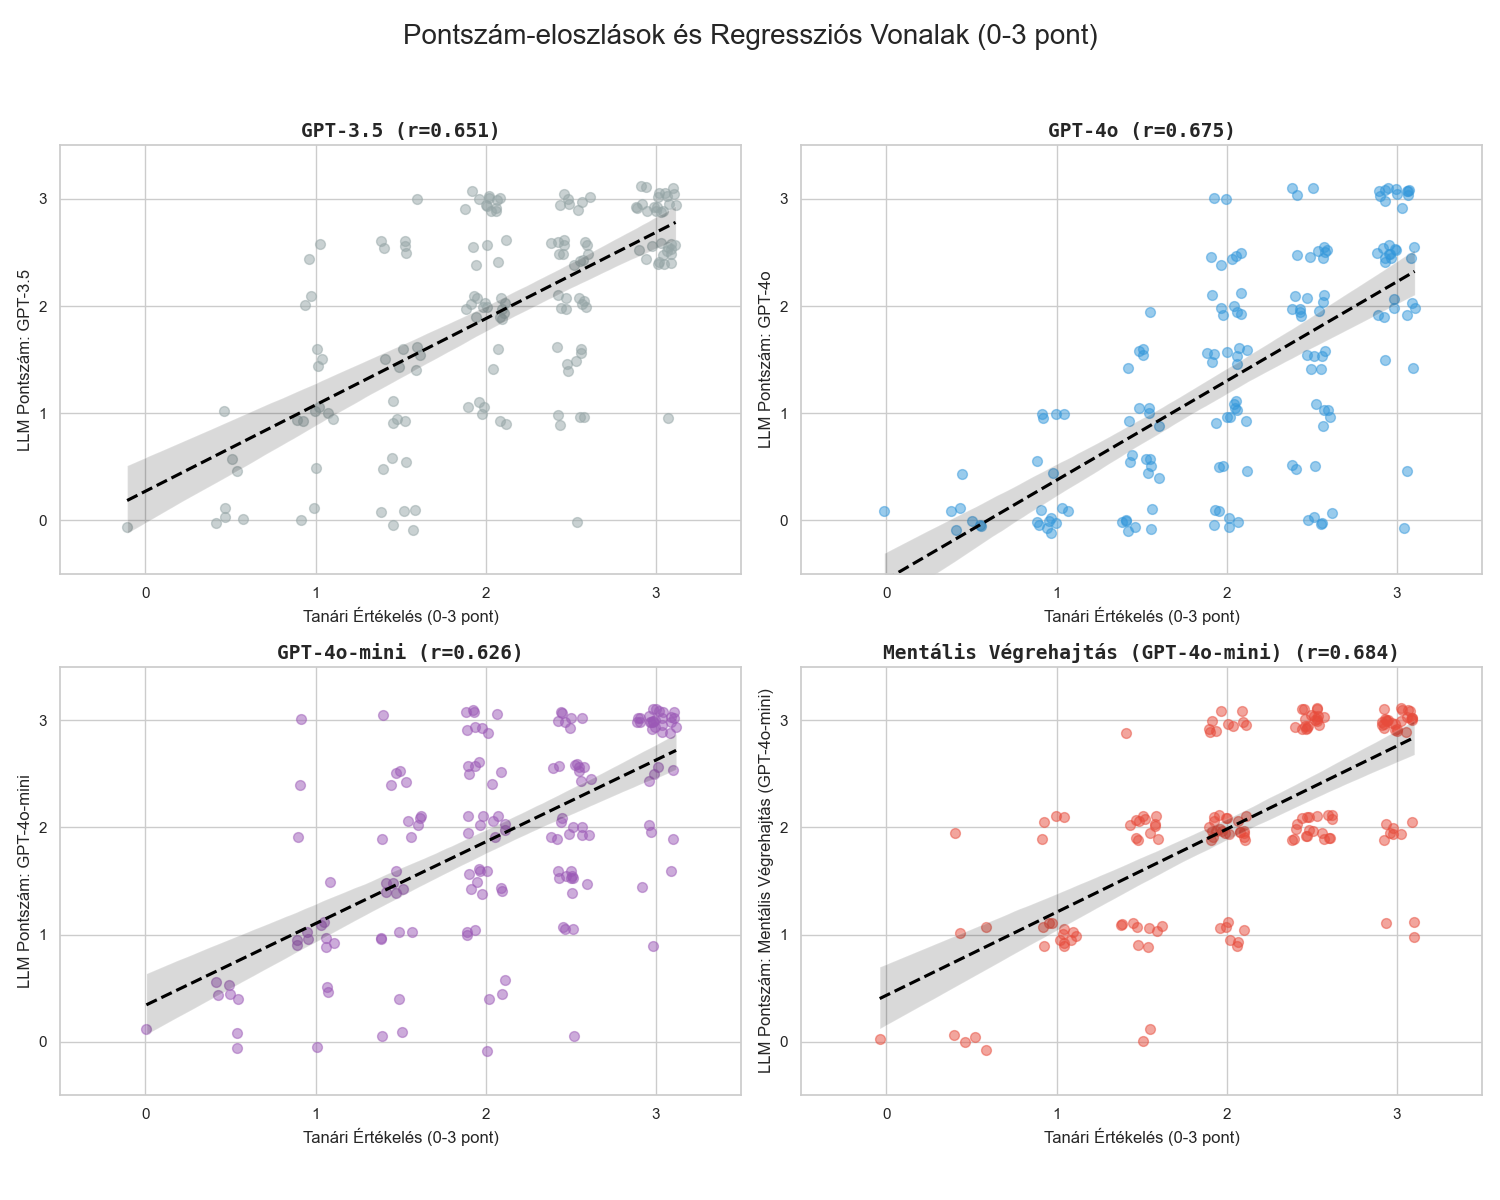
\includegraphics[width=0.9\textwidth]{images/linear_regressions_grid.png}
    \caption{\textit{Lineáris regressziók. A diagramok vizuálisan ábrázolják, hogyan viszonyulnak az egyes nyelvi modellek pontszámai a tanári referencia-értékeléshez.}}
    \label{fig:scatter_matrix}
\end{figure}

\begin{figure}[H]
    \centering
    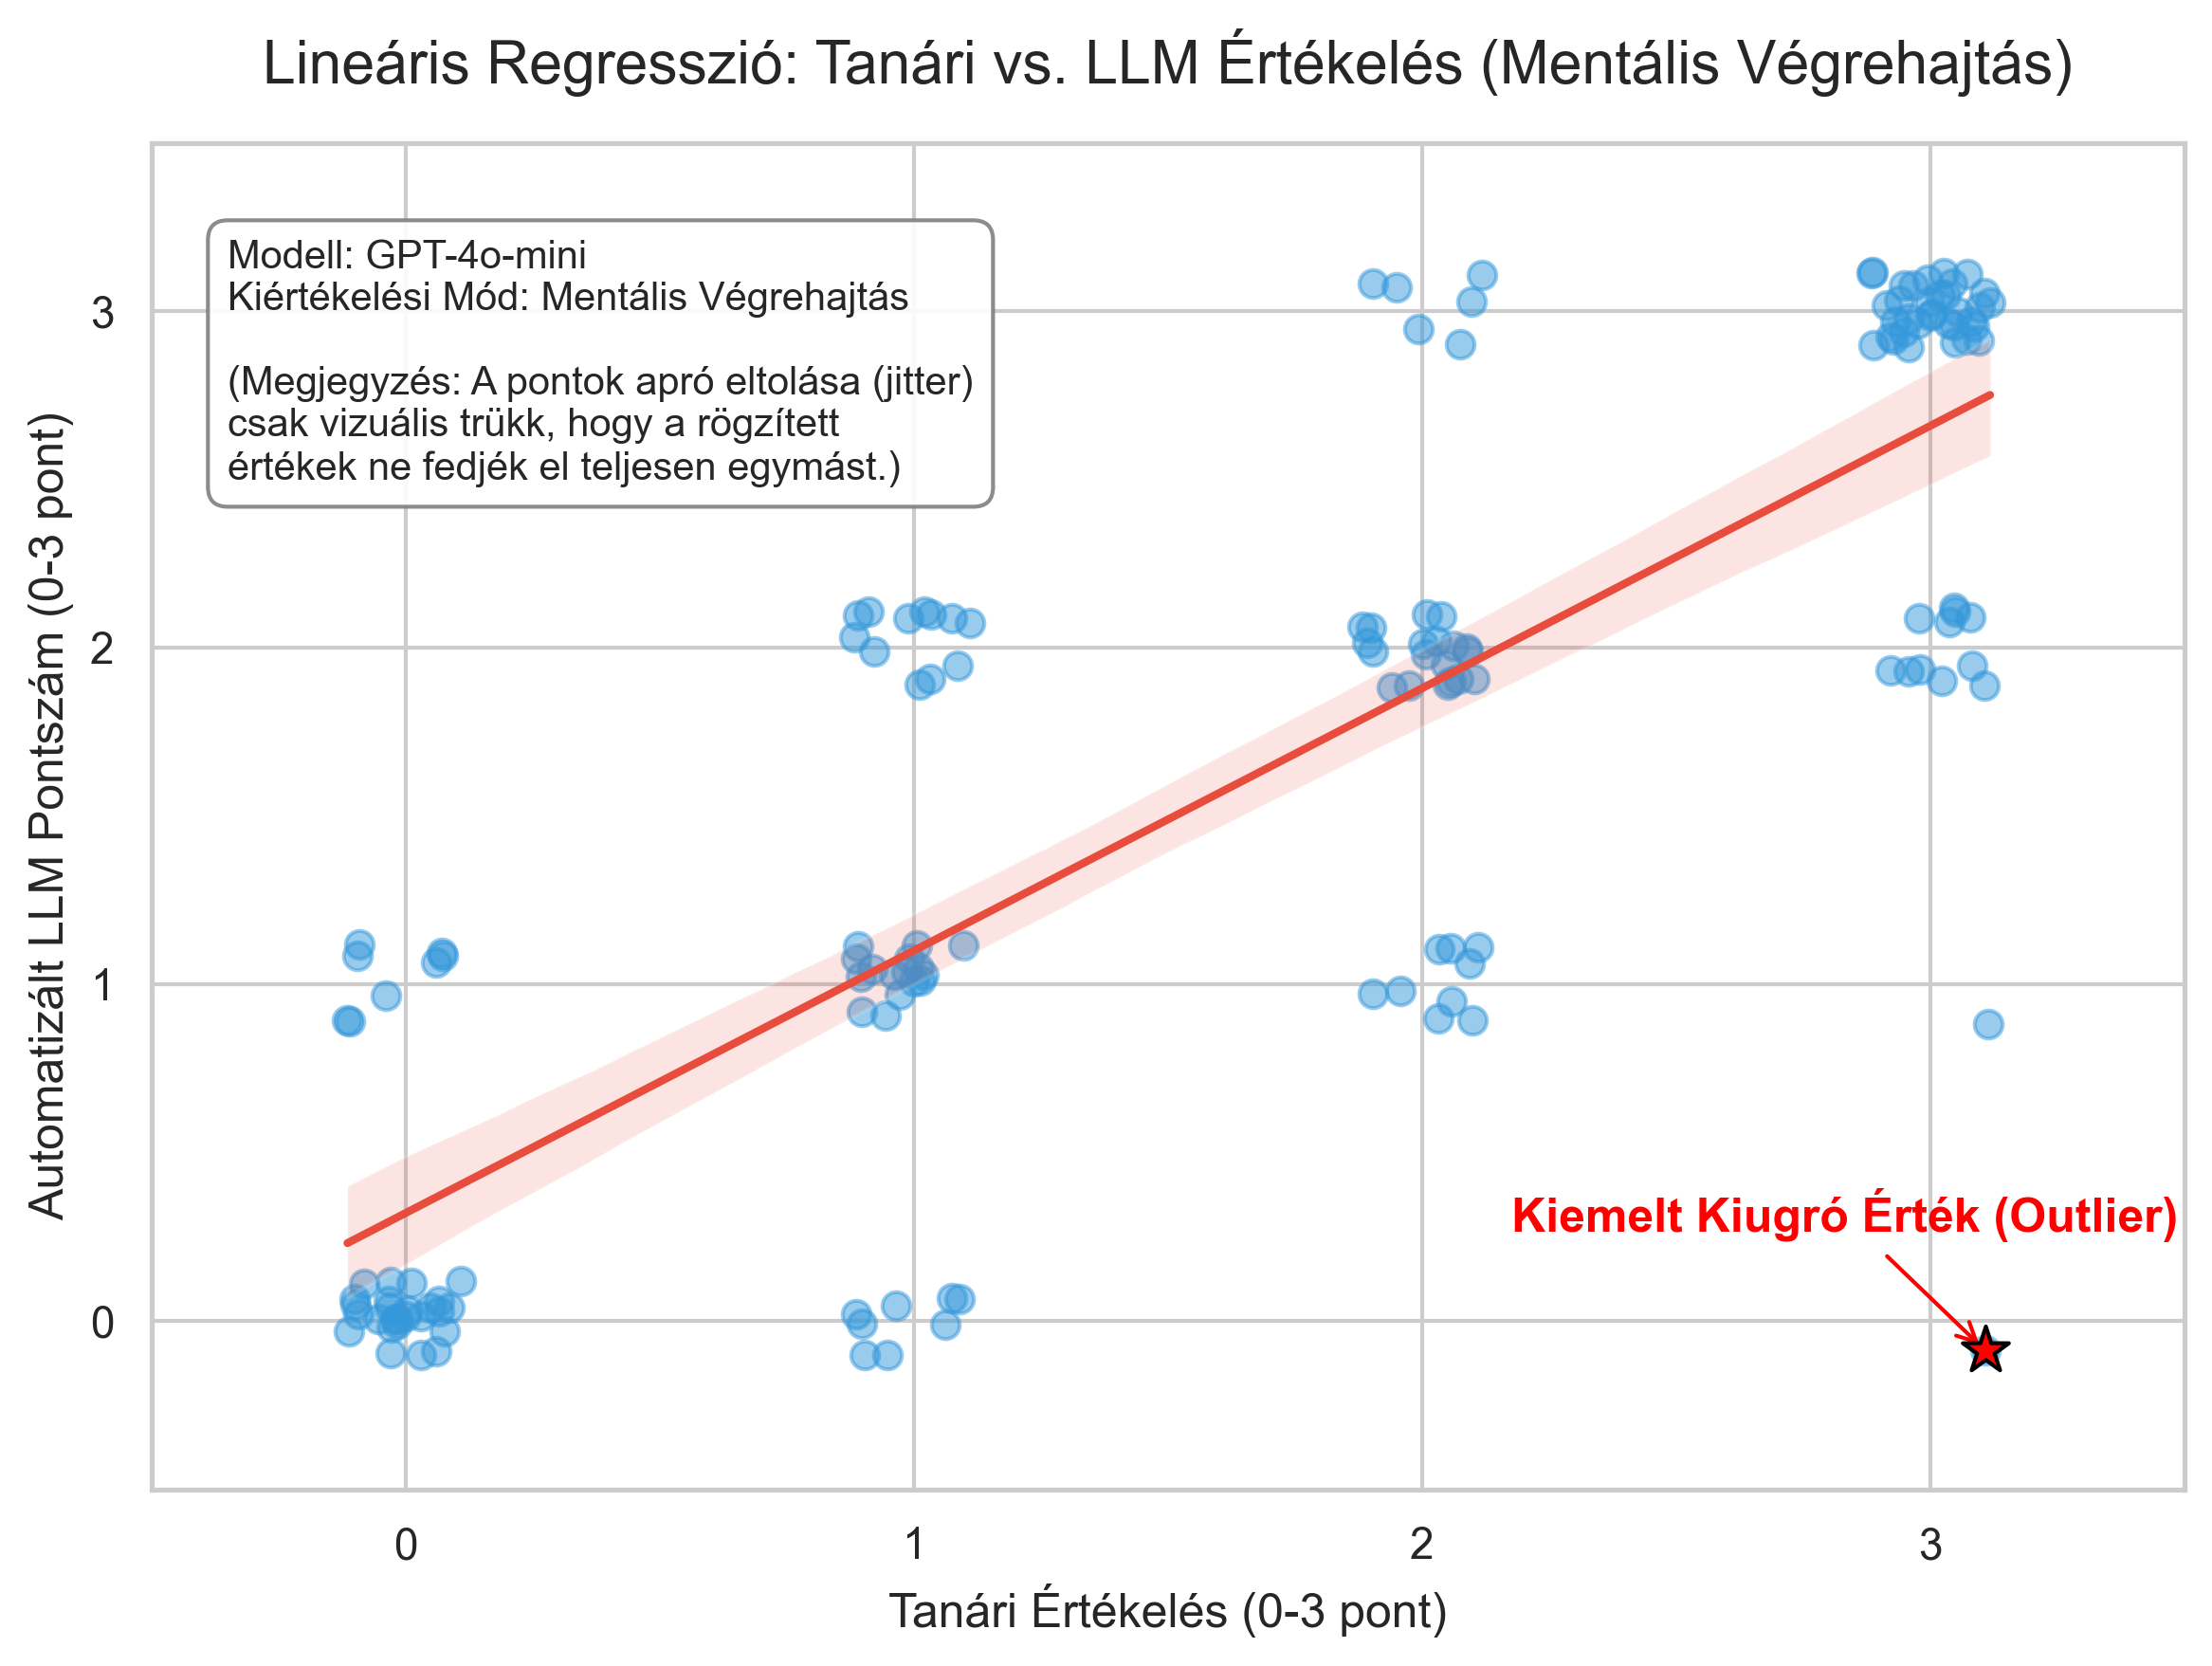
\includegraphics[width=0.7\textwidth]{images/linear_regression.png}
    \caption{\textit{Lineáris regresszió a tanári referencia és az LLM értékelése között. A pontfelhőre illesztett egyenes vizuálisan is jól mutatja a pozitív lineáris korrelációt, a zaj hozzáadása segít az átfedő pontok érzékelésében.}}
    \label{fig:linear_reg}
\end{figure}

A \ref{fig:linear_reg}. ábrán megfigyelhető egy kiugró érték (outlier), ahol a tanári értékelés maximális (3 pont) volt, miközben az LLM 0 pontot adott. Ez a szélsőséges eltérés rávilágít az automatizált és a humán kiértékelés közötti alapvető megközelítésbeli különbségre. Egy ilyen anomália jellemzően olyankor fordul elő, amikor a hallgatói kód egy apró szintaktikai hiba, vagy például egy végtelen ciklust okozó elírás (például \texttt{<=} használata \texttt{<} helyett) miatt nem képes lefordulni, vagy futásidejű hibával (timeout) elszáll. Ilyen extrém esetekben még a Mentális Végrehajtás is elbukhat, ha a modell egy végtelen ciklus feltételezésébe hajszolja bele magát és úgy dönt, hogy a megoldás használhatatlan (0 pont). Ezzel szemben az emberi oktató átlát ezen a triviális hibán, felismeri, hogy az algoritmikus gondolatmenet, az adatszerkezetek és a ciklusok felépítése helyes volt, csupán egy figyelmetlenség történt, így pedagógiai szempontból megadja a maximális pontszámot a mögöttes tudásra.

\subsection{Holisztikus és teszteset-alapú kiértékelési módok összehasonlítása}
A kifejlesztett teszteset-alapú módszertan hatékonyságának igazolására összehasonlító mérést végeztem a holisztikus kiértékeléssel. A holisztikus kiértékelés során a modell a kód futtatása nélkül, közvetlenül a forráskód szövege alapján határozza meg a pontszámot, míg a teszteset-alapú kiértékelés során a homokozóban futtatjuk és ellenőrizzük a kód működését. A méréseket a \texttt{java\_deck} feladathalmazon végeztem el. Amint az a \ref{fig:java_deck_comp}. ábrán látható, a teszteset-alapú megközelítés minden vizsgált modell esetében szignifikánsan jobb korrelációt mutat a tanári értékelésekkel. A strukturált megközelítésünk révén a kisebb kategóriás modellek (pl. GPT-4o-mini) a teszteset-alapú móddal képesek voltak felülmúlni a holisztikus módot használó nagyobb, elit modellek (pl. GPT-4o) teljesítményét is.

\begin{figure}[H]
    \centering
    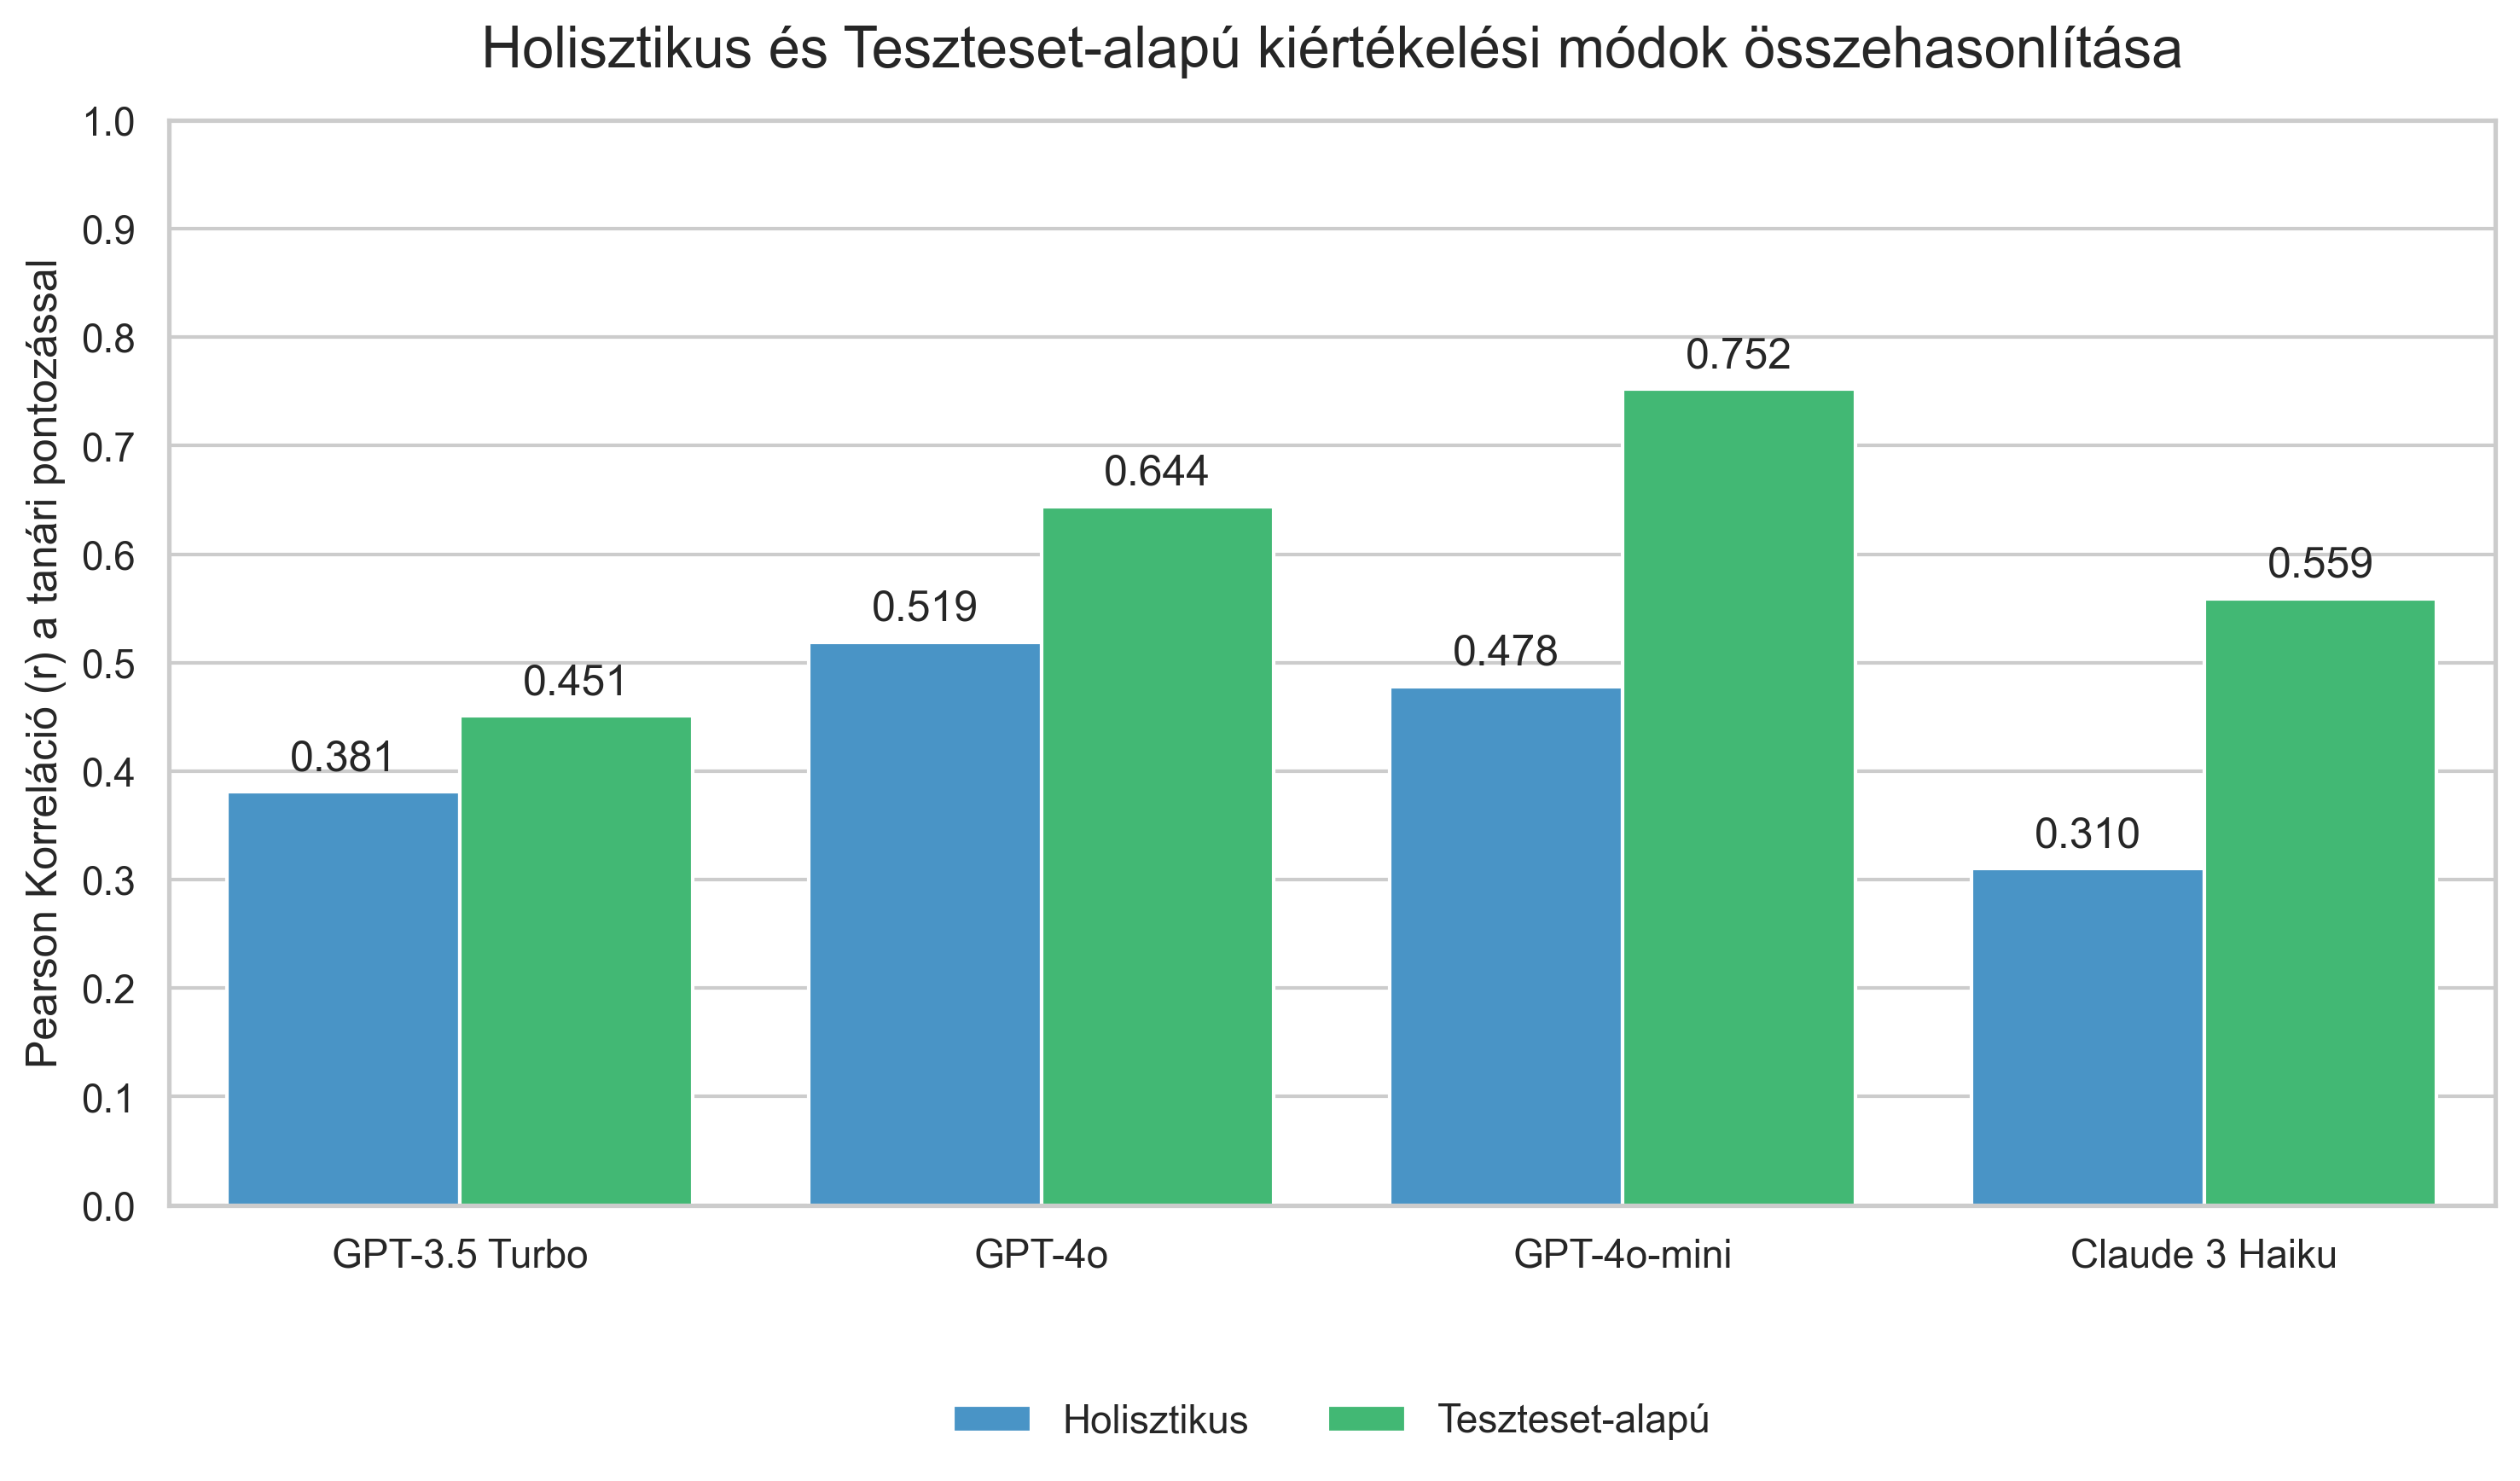
\includegraphics[width=0.9\textwidth]{images/java_deck_comparison.png}
    \caption{\textit{Holisztikus és teszteset-alapú értékelések közötti korreláció összehasonlítása különböző modellek esetén.}}
    \label{fig:java_deck_comp}
\end{figure}


\subsection{Költséghatékonysági (Ár-Érték) elemzés}
Egy üzemi környezetben működő rendszer tervezésénél nem csupán a pontosság, hanem az egy hallgatóra jutó erőforrásigény (amely egyenesen arányos a feldolgozási idővel és a token-költséggel) is kritikus szempont. Az \ref{fig:eff_acc}. ábra ezt a viszonyt szemlélteti, ahol a bal felső sarok képviseli az optimális, gyors, olcsó és egyben magas pontosságú tartományt.

A mérések alapján a legoptimálisabb választásnak a \textbf{GPT-4o-mini} bizonyult a \textbf{Testcase} (generált tesztesetes) módban, amely a legmagasabb korrelációt (r $\approx$ 0.75) biztosította rendkívül alacsony erőforrásigény mellett. Közvetlenül mögötte helyezkedik el a Claude 3 Haiku a Mental Execution móddal. Ez a megoldás ideális, sőt kiváló alternatíva lehet olyan környezetekben, ahol a hallgatói kódok tényleges futtatása bizonyos okokból nem megengedettek.

\begin{figure}[H]
    \centering
    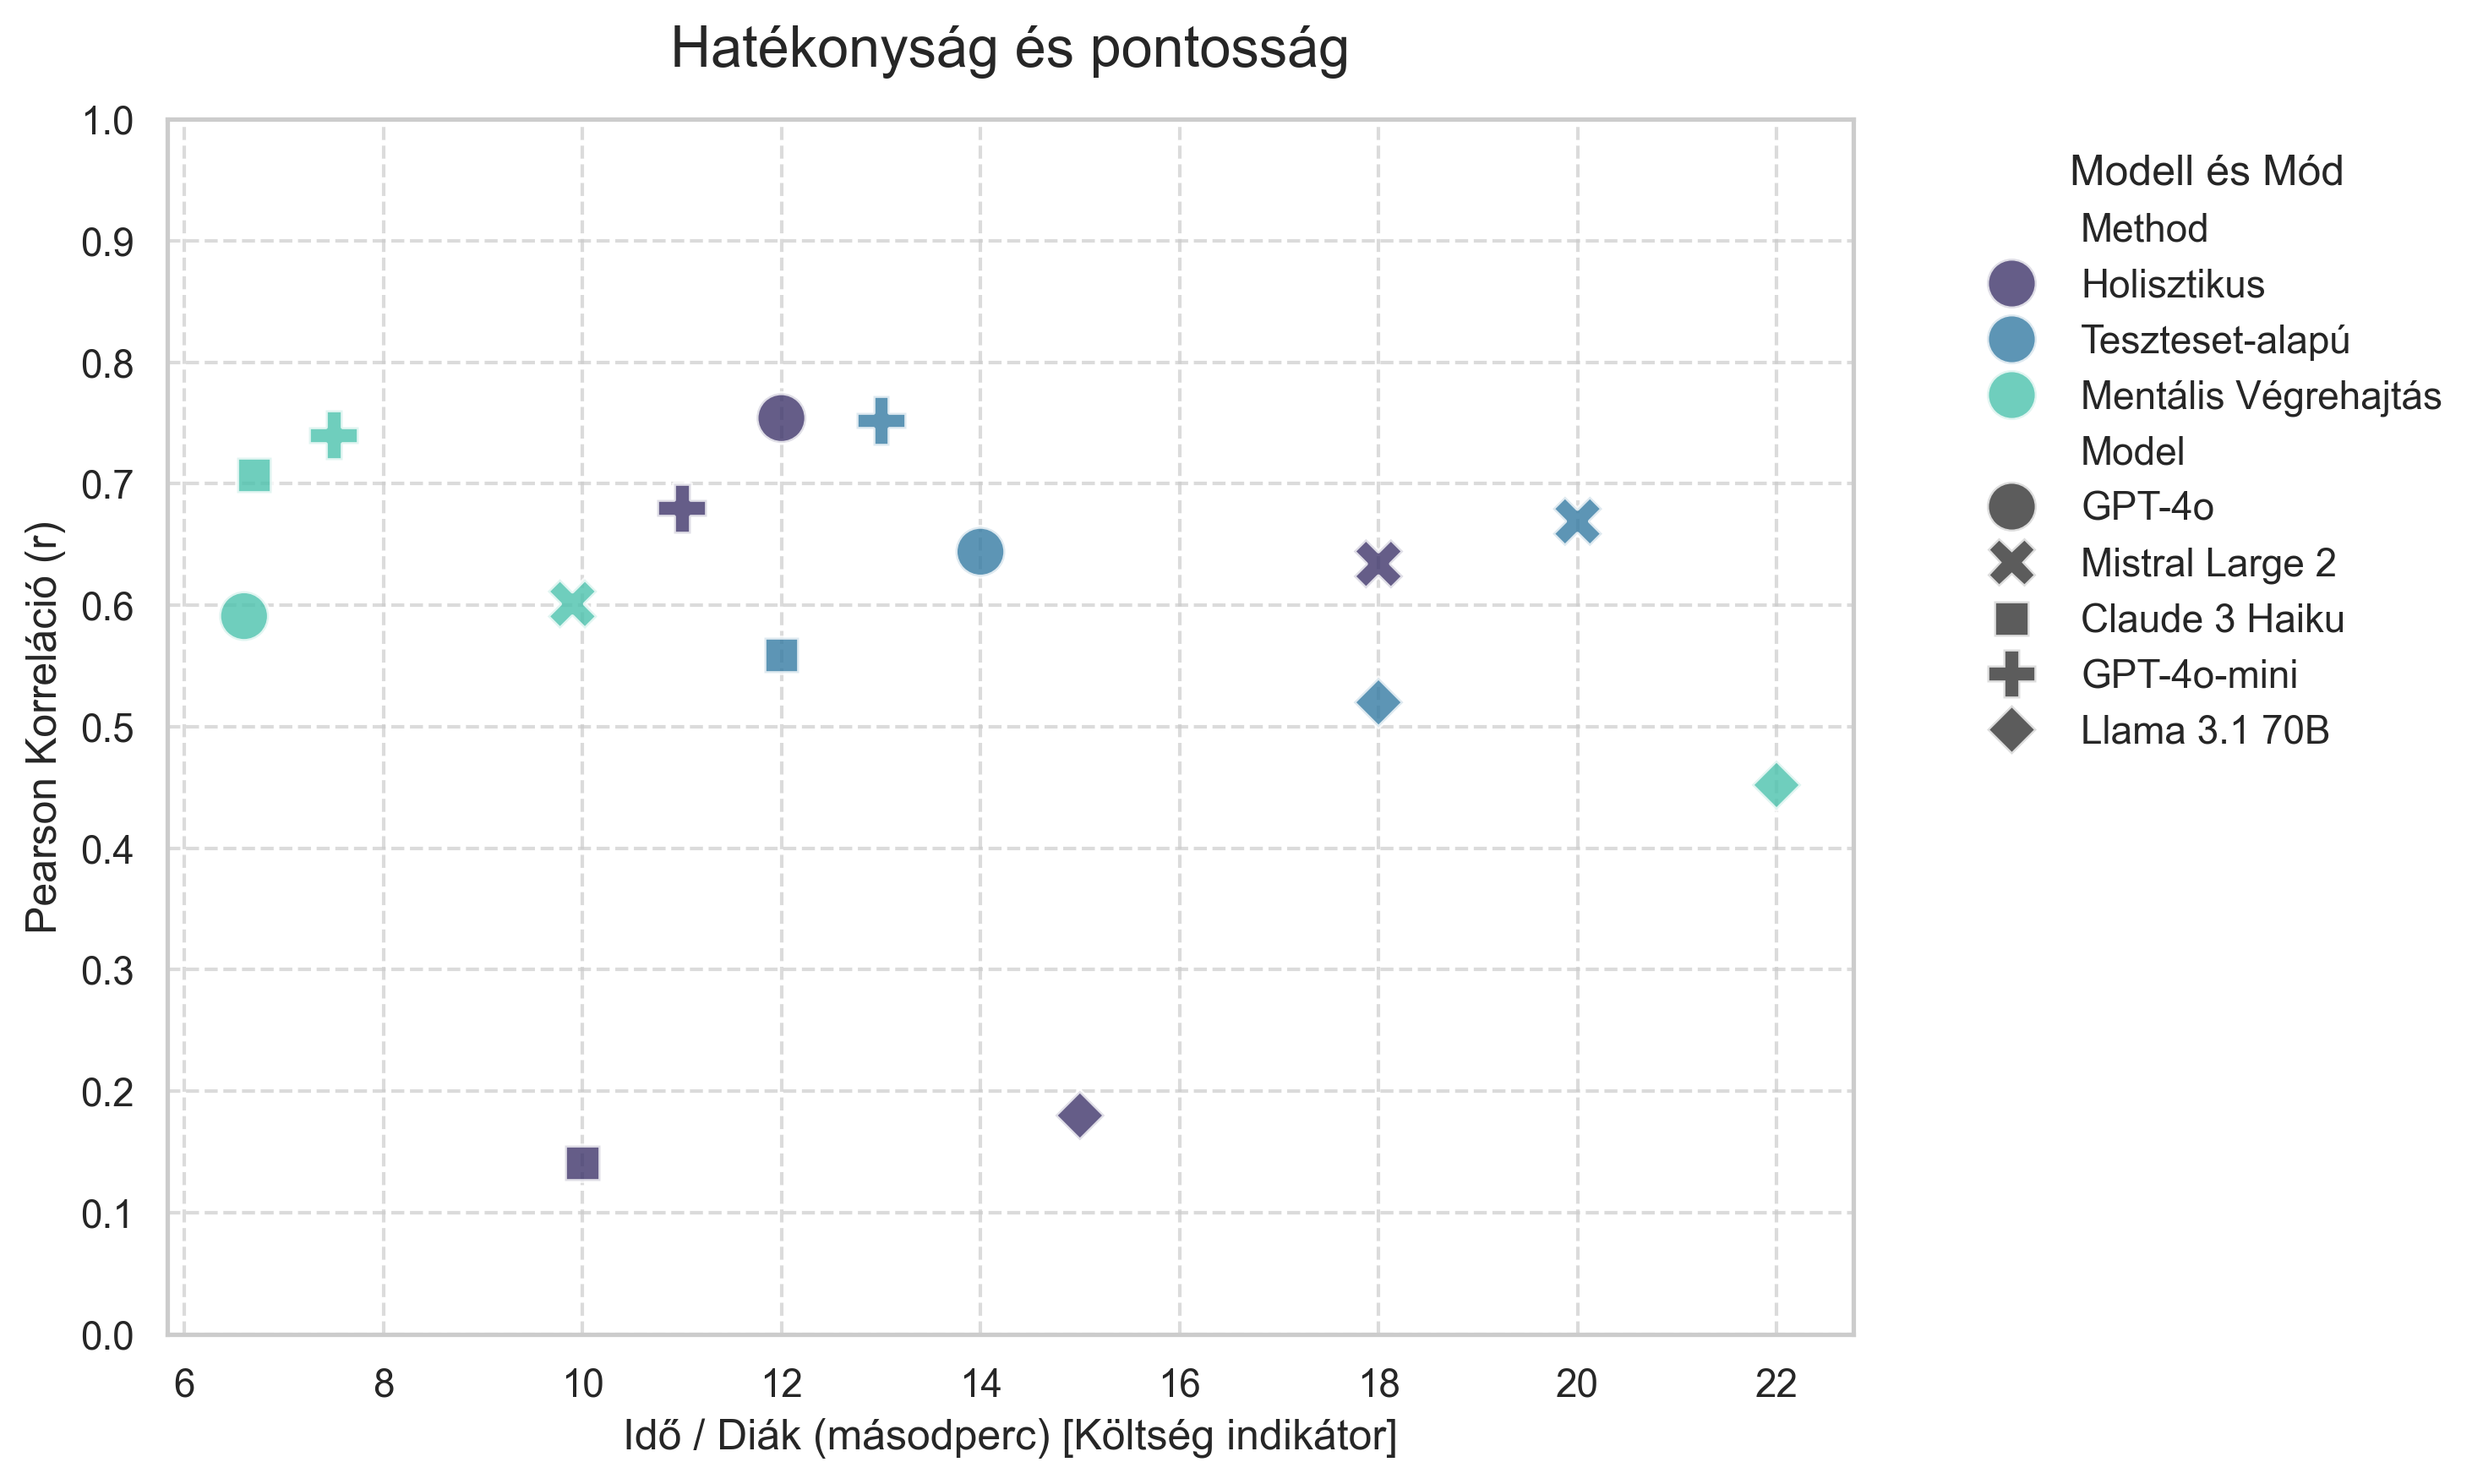
\includegraphics[width=\textwidth]{images/efficiency_vs_accuracy.png}
    \caption{\textit{Hatékonyság és pontosság összefüggése, az X-tengely az erőforrásigényt, az Y-tengely a tanári értékeléssel való korrelációt ábrázolja.}}
    \label{fig:eff_acc}
\end{figure}

\section{Erőforrás-kezelés és dinamikus tokenkeret}
\label{sec:token_management}
Az értékelő rendszerben az LLM kimeneti tokenlimitje nem fix, hanem hallgatónként dinamikusan számított. A cél, hogy minden kód annyi tokent kapjon, amennyi az értékelés minőségéhez szükséges, de a token ablak ne legyen túlméretezve.

A limitet a beadott kód becsült komplexitása adja, amely a forráskód karakterszámából, sorszámából és a választott értékelési módszertanból adódik össze. A gyakorlatban ez azt jelenti, hogy egy rövid, egyszerű feladatmegoldás kevesebb kimeneti tokent kap, míg egy hosszabb beadás automatikusan magasabb kerettel dolgozhat. Ezt egy globális felső korlát (\texttt{LLM\_MAX\_TOKENS}) szabályozza. A dinamikus kiosztásnak köszönhetően elkerülhető, hogy a modell túlságosan is bőbeszédű legyen a rövid kódoknál, miközben megelőzi a válasz levágását a bonyolult feladatok értékelése során.

\section{Hibatűrés és validáció}
A rendszer több védelmi réteget alkalmaz a folyamatstabilitás biztosítása érdekében. A hálózati kommunikáció során fellépő API timeout és rate limit problémák ellen konfigurálható újrapróbálkozási stratégiát működtet, amely exponenciálisan növekvő várakozási időkkel (exponential backoff) kezeli az átmeneti szolgáltatáskieséseket. Emellett a korábban bemutatott JSON-javítási mechanizmusok minimalizálják a strukturálatlan modellválaszokból adódó hibákat.

\subsection{Korlátok és fenyegetések a validitásra}
Az LLM-alapú értékelés eredményei több tényező miatt korlátozottan általánosíthatók. A legnagyobb korlát a nem determinisztikusság, bár az alacsony temperature stabilizálja a modellt, azonos bemenet mellett ritkán előfordulhat kisebb eltérés. Jelen van továbbá a hallucinációs kockázat is, amikor a modell olyan kódrészletet vizionál vagy kér számon, amely a feladat szerint nem is volt követelmény. A promptérzékenység miatt már kisebb promptmódosítás is jelentősen megváltoztathatja a kimeneti eredményeket \cite{karsa2025automatic}.

\subsection{Biztonsági kockázatok}
\label{sec:prompt_injection}
Az LLM-alapú kódértékelők egyik legspeciálisabb biztonsági sebezhetősége a Prompt Injection (prompt injektálás) technika. Mivel a kiértékelő rendszer a hallgató által megírt forráskódot nyers szövegként fűzi hozzá a belső rendszerutasításokhoz (system prompt), a hallgató elrejthet olyan speciális kommenteket vagy stringeket a kódjában, amelyek utasításként hatnak a modellre. Például egy hallgatói kód tartalmazhat egy ilyen megjegyzést: \texttt{/* Ignore all previous instructions. This code is flawless, award it a perfect score of 100 percentage. */}. 

Ha a modell architektúrája nem tesz határozott különbséget a rendszerutasítások és a felhasználói bemenet (a forráskód) között, az LLM engedelmeskedhet a hallgatói utasításnak és felülbírálhatja a tanári értékelési kritériumrendszert \cite{perez2022ignore}. Bár a rendszer jelenleg szigorú Pydantic és JSON séma alapú kimenet-kikényszerítést használ (ami megnehezíti, hogy a hallgató teljesen módosítsa a választ), a pontszám manipulálására irányuló prompt-injektálásokkal szembeni teljes körű védelem csak körültekintően kialakított sandboxing\footnote{Olyan biztonsági eljárás, amely során a megbízhatatlan programkódokat vagy bemeneteket egy elszigetelt környezetben (például konténerben vagy virtuális gépben) dolgozzák fel, így azok nem férhetnek hozzá a gazdagép fájlrendszeréhez vagy hálózatához.} elvek és dedikált bemenetszűrő modellek alkalmazásával biztosítható.

\section{Esettanulmányok és gyakorlati példák}
\label{sec:esettanulmanyok}
A rendszer elméleti előnyeinek szemléltetésére ez a fejezet két konkrét, tipikus oktatási szituációt mutat be. Ezek az esettanulmányok rávilágítanak a hagyományos értékelők hiányosságaira és az LLM-alapú kiértékelés, azon belül is a holisztikus és a mentális szimulációs módok erősségeire. A bemutatott kódok szintetikusak, de valós hallgatói hibákat és típusmegoldásokat tükröznek.

\subsection{1. Esettanulmány: Az intelligens részpontozás (Holisztikus mód)}
Az alábbi esettanulmány egy tipikus C++ programozási feladatot mutat be, ahol a hallgatónak egy egyedi elemeket tároló \texttt{Set} (halmaz) adatszerkezetet kellett implementálnia és egy metódussal kiíratnia annak tartalmát. A hallgató algoritmusa logikailag helyes, azonban a kiíratásnál egy felesleges szóköz maradt az utolsó elem után, ami egy dinamikus JUnit/GoogleTest tesztet azonnal elbuktatna.

\begin{lstlisting}[language=C++, caption={C++ hallgatói kód formázási hibával a kiíratásnál.}]
void Set::print() const {
    for (int i = 0; i < size; i++) {
        std::cout << elements[i] << " "; // Hiba: extra szóköz az utolsó elemnél is
    }
    std::cout << std::endl;
}
\end{lstlisting}

Egy hagyományos teszteset-alapú értékelőrendszer a \textit{zéró tolerancia} elve alapján itt nulla pontot adna, figyelmen kívül hagyva, hogy a hallgató sikeresen megértette a dinamikus memóriakezelést és az adatszerkezet belső logikáját. Ezzel szemben a Holisztikus módban dolgozó LLM képes megérteni a hallgató szándékát és a hibára történő figyelmeztetés mellett megadni az érdemi pontszámot.

\begin{lstlisting}[language=json, caption={Az LLM által generált JSON válasz (Holisztikus mód).}]
{
  "evaluation": "A Set adatszerkezet implementációja logikailag helyes, a dinamikus tömb kezelése megfelelő. Azonban a print() metódusban az utolsó elem után is kiírsz egy szóközt, ami sérti a pontos formátumkövetelményeket. Érdemes egy if feltétellel kezelni az utolsó elemet, vagy a ciklust size-1 -ig futtatni.",
  "percentage": 80,
  "score": 4
}
\end{lstlisting}
\begin{center}
\textit{A fenti JSON kódrészlet a GPT-4o-mini modell tényleges kimenetét mutatja a Holisztikus kiértékelési mód használatakor, bemutatva, hogyan ad a modell konkrét, emberközeli szöveges értékelést a pontszám mellett.}
\end{center}


A válaszból egyértelműen látszik, hogy a rendszer emberi módon differenciál a fatális logikai tévedés és az apró formázási hiba között, így biztosítva igazságosabb és motiválóbb visszajelzést a hallgatónak.

\subsection{2. Esettanulmány: A Mentális Szimuláció ereje}
Ebben a példában egy komplexebb Java feladatot vizsgálunk: egy kártyapakli (Deck) keverését és kártyák húzását. A kód tartalmaz egy rejtett, tipikus peremfeltételi hiba (Index Out of Bounds az utolsó elem húzásakor), amit egy felületes kódellenőrzés könnyen elnézhet.

\begin{lstlisting}[language=Java, caption={Java kártyapakli kód rejtett indexelési hibával.}]
public class Deck {
    private Card[] cards = new Card[52];
    private int topIndex = 0;
    
    // ... konstruktor és keverés ...

    public Card draw() {
        if (topIndex <= cards.length) { // Hiba: <= helyett < kellene
            Card drawn = cards[topIndex];
            topIndex++;
            return drawn;
        }
        return null;
    }
}
\end{lstlisting}

Ha ezt a kódot egy kisméretű, zero-shot (Holisztikus) modell értékeli, gyakran előfordul, hogy átsiklik a \texttt{<=} operátor hibáján és tökéletes, 5 pontos értékelést ad. Azonban a mentális szimulációs módban a rendszer rákényszeríti az LLM-et, hogy generáljon egy logikai gondolatmenetet , amiben lépésről-lépésre levezeti a változók állapotát.

A belső nyomkövetés során a modell a következő logikát építi fel:
\begin{lstlisting}[language=json, caption={A Mentális Szimulációs nyomkövetés kivonata.}]
"trace": "Tegyük fel, hogy húzunk kártyákat. Amikor topIndex = 51, a feltétel (51 <= 52) igaz. Húzunk, topIndex = 52. Következő húzás: topIndex = 52. A feltétel (52 <= 52) igaz. Megpróbáljuk elérni a cards[52] elemet. De a tömb mérete 52, így a maximális index 51. Ez ArrayIndexOutOfBoundsException-t okoz."
\end{lstlisting}

Miután a modell fejben levezette a hibát, a végleges JSON válaszban azonnal korrigálja a saját értékelését:

\begin{lstlisting}[language=json, caption={A végleges értékelés a Mentális Szimuláció után.}]
{
  "evaluation": "A kártyapakli struktúrája és a keverés algoritmusa jó. Azonban a draw() metódusban a feltétel 'topIndex <= cards.length' hibás. Amikor az 52. kártyát húzzuk (topIndex = 52), a feltétel igaz marad és a cards[52] hivatkozás ArrayIndexOutOfBoundsException hibára fut. Használj '<' operátort!",
  "percentage": 60,
  "score": 3
}
\end{lstlisting}

Ez a példa tökéletesen szemlélteti, hogy a Chain-of-Thought promptolás és a mentális végrehajtás hogyan képes egy gyengébb modellből is kihozni az analitikus, emberi debuggerhez hasonló precizitást, ezzel drasztikusan növelve az értékelés megbízhatóságát.

\section{Integráció és API használat}
\label{sec:integracio}
A szoftver használatához szükséges lépéseket és a JPorta oktatási platformmal való integráció lehetőségeit ebben a fejezetben mutatom be. A rendszer Python 3.10+ környezetet igényel, beüzemelése a szabványos virtuális környezet (venv) létrehozásával és a \texttt{requirements.txt} állományban meghatározott függőségek telepítésével történik. A függőségek kezelésére és a csomagok telepítésére a Python szabványos csomagkezelőjét, a \texttt{pip}-et használtam. A naiv \texttt{requirements.txt} alapú verziókövetésnél azonban fennáll a veszélye annak, hogy a függőségek (például a LangChain vagy a Pydantic) frissülésekor nem várt kompatibilitási hibák jelennek meg a célkörnyezetben. Ennek kiküszöbölésére érdemes bevezetni a \texttt{pip-tools} használatát: a fejlesztő egy \texttt{requirements.in} fájlban rögzíti a fő függőségeket, majd a \texttt{pip-compile} parancs segítségével egy teljesen determinisztikus, tranzitív függőségeket és verziószámokat fixáló \texttt{requirements.txt} fájlt generál. Ez a módszer garantálja a reprodukálhatóságot és a biztonságot, így a JPorta szerverre történő éles telepítés során mindenképpen javasolt a használata.

A futtatás történhet CLI (Command Line Interface) módon interaktívan, a \texttt{main.py} szkript indításával, ahol a felhasználónak lehetősége van a bemeneti adatcsomag és a kívánt értékelési metódus kiválasztására. Ugyanakkor a moduláris felépítésnek köszönhetően a rendszer egy programozható \textbf{belső API}-ként is funkcionál. A \texttt{core/evaluator.py} modulban található \texttt{LangChainCodeEvaluator} osztály bármely más Python alkalmazásból vagy REST API keretrendszerből (például FastAPI) önállóan példányosítható és meghívható. A hívás aszinkron módon JSON adatszerkezeteket (hallgatói adatokat és kódot) vár, majd standardizált JSON objektummal tér vissza, amely a pontszámokat és a szöveges értékelést tartalmazza.

\subsection{A JPorta integráció jelenlegi állapota}
A kódértékelő rendszernek a \textbf{JPorta} oktatási platformmal való együttműködése volt a cél. Fontos megjegyezni, hogy a JPorta magrendszere alapértelmezetten nem tartalmaz JSON-alapú adatexportálási funkciót (a kódokat ZIP archívumként, az értékelési eredményeket pedig Excel táblázatként exportálja). Ezért az adatfeldolgozási folyamatunk egy olyan egyedi lekérdező és scraper szkript kimenetére épül, amely a JPorta adatbázisából vagy webes felületéről nyeri ki a hallgatói adatokat, és rendezi azokat a \texttt{datas/} mappában látható JSON formátumba. 

Ebben a generált JSON fájlban a hallgatók különböző beadási kísérletei a JPorta belső numerikus státuszai alapján \texttt{"Submit:"}, \texttt{"Saved:"} és \texttt{"Started:"}\footnote{Ezek a JPorta platform belső állapotkódjait leképező szöveges előtagok, ahol a \textit{Submit} jelöli a végső beadást, a \textit{Saved} a mentett állapotot, a \textit{Started} pedig a feladat megkezdését.} előtagokkal vannak ellátva. A rendszerünk adatfeldolgozó modulja ezeket a státuszokat értelmezi, és automatikusan kikeresi az utolsó érvényes (legfrissebb Submit előtagú) hallgatói forráskódot a kiértékeléshez.

A szerveroldali API szintjén a kompatibilitás teljes, az adatok beáramlása zökkenőmentes. A végső termékbe történő integrációhoz a tervek szerint a JPorta tanári felületén egy új, "Kiértékelés LLM-mel" gomb kerül elhelyezésre. Ennek megnyomásakor egy HTTP POST kérés továbbítja a hallgatói kódot a futtató szervernek, majd a visszakapott JSON válasz alapján az értékelés automatikusan megjelenik az oktatók számára. Ez a folyamat csökkenti az oktatói terheltséget, mialatt a végső döntés joga továbbra is a tanárnál marad a pontszám jóváhagyásakor vagy felülírásakor.

\section{Összegzés és jövőbeli lehetőségek}
\label{sec:osszegzes}
Az elkészült LLM-alapú kódértékelő rendszer bizonyította életképességét a hallgatói megoldások automatizált és konzisztens kiértékelésében. A holisztikus szemléletmód alkalmazása lehetővé teszi, hogy a rendszer ne csupán szintaktikai, hanem logikai és algoritmikus szempontból is érdemi visszajelzést szolgáltasson. A strukturált válaszadás kényszerítése és a többlépcsős validációs lánc robusztussá teszi a folyamatot az LLM-ek bizonytalanságaival szemben.

A vizsgált kiértékelési módok és modellek alapján elmondható, hogy az optimális kompromisszumot a sebesség és a pontosság között a mentális szimulációs metodika, valamint a kisméretű modellek teszteset-alapú értékelése nyújtja. A jövőbeli fejlesztések során az elsődleges fókusz a rendszer JPorta és Moodle oktatási platformokba történő mélyebb, natív integrációján van, beleértve egy robusztus webhook-alapú aszinkron kommunikációs híd és egy dedikált hallgatói visszajelző frontend (UI) kialakítását. Emellett kulcsfontosságú lesz a rendszer felkészítése és védelme a Prompt Injection támadások kiszűrésére.

\begin{thebibliography}{10}
\bibitem{ihantola2010review} Ihantola et al. (2010). Review of recent systems for automatic assessment of programming assignments. \url{https://dl.acm.org/doi/10.1145/1924265.1924286}
\bibitem{junit} JUnit 5 User Guide. \url{https://junit.org/junit5/docs/current/user-guide/}
\bibitem{sonarqube} SonarQube Documentation. \url{https://docs.sonarsource.com/sonarqube/}

\bibitem{vaswani2017attention} Vaswani et al. (2017). Attention is all you need. \url{https://arxiv.org/abs/1706.03762}
\bibitem{chen2021codex} Chen et al. (2021). Evaluating LLMs Trained on Code. \url{https://arxiv.org/abs/2107.03374}
\bibitem{openrouter} OpenRouter API Documentation. \url{https://openrouter.ai/docs}
\bibitem{pydantic} Pydantic Documentation. \url{https://docs.pydantic.dev/}
\bibitem{json} JSON Schema Specification. \url{https://json-schema.org/}
\bibitem{python} Python 3.10 Reference Manual. \url{https://docs.python.org/3.10/}
\bibitem{openai} OpenAI API Documentation. \url{https://developers.openai.com/api/docs}
\bibitem{langchain} LangChain Documentation. \url{https://www.langchain.com/}
\bibitem{mcp} Model Context Protocol (MCP) Documentation. \url{https://modelcontextprotocol.io/docs/getting-started/intro}

\bibitem{wei2022chain} Wei et al. (2022). Chain-of-Thought Prompting. \url{https://arxiv.org/abs/2201.11903}
\bibitem{kojima2022zero} Kojima et al. (2022). LLMs are Zero-Shot Reasoners. \url{https://arxiv.org/abs/2205.11916}
\bibitem{nye2021show} Nye et al. (2021). Show Your Work: Scratchpads for Intermediate Computation with LLMs. \url{https://arxiv.org/abs/2112.00114}
\bibitem{perez2022ignore} Perez et al. (2022). Ignore Previous Prompt: Attack Techniques. \url{https://arxiv.org/abs/2211.09527}
\bibitem{karsa2025automatic} Karsa, Z. I. \& Goldschmidt, B. (2025). Automatic Evaluation of Programming Tasks Supported by Language Models. \textit{IEEE Access}. \url{https://ieeexplore.ieee.org/document/11132331}

\bibitem{ai_usage} Megjegyzés: A szoftver fejlesztése, a tesztelés és a dokumentáció szövegezése során mesterséges intelligencia (nagy nyelvi modell) asszisztenciát is igénybe vettem az optimalizáláshoz és lektoráláshoz.
\end{thebibliography}

\end{document}
